\begin{ledgroupsized}[r]{120mm}
\footnotesize
\pstart
\noindent\textbf{\"{U}berlieferung:}
\pend
\end{ledgroupsized}
%
\begin{ledgroupsized}[r]{114mm}
\footnotesize
\pstart
\parindent -6mm
\makebox[6mm][l]{\textit{L}}%
Auszüge mit Bemerkungen aus \cite{00311}E. \textsc{Mariotte}, \textit{Traité de la percussion ou chocq des corps}, Paris 1673:
LH XXXV 14, 2 Bl. 112-115. 2 Bog. 2\textsuperscript{o}.
4\,\nicefrac{3}{4} S. Textfolge: Bl. 115~r\textsuperscript{o}, 115~v\textsuperscript{o}, 112~r\textsuperscript{o}, 112~v\textsuperscript{o}, 113~r\textsuperscript{o}, 113~v\textsuperscript{o}.
Am Anfang von Bl. 112~r\textsuperscript{o} Leibniz' eigenhändiger Kustos: \textit{Continuatio Excerptorum ex libro Mariotti de la percussion.}
Bl. 114 sowie die ersten \nicefrac{3}{4} von Bl. 115~r\textsuperscript{o} überliefern N.~9. %?? = ex 10 = LH 35.14.02, 114-115 = Wallis-2
Die untere Hälfte von Bl. 113~v\textsuperscript{o} ist leer.
Auf Bl. 115~v\textsuperscript{o} findet sich ferner N.~80. %?? = ex 81 = LH 35.14.02, 112-115 = Einkaufsliste
Bis zum letzten Viertel von Bl. 112~v\textsuperscript{o} besteht das vorliegende Stück aus Exzerpten;
danach weist der Text eigenständigen Charakter auf, was auch auf verschiedene Entstehungszeiten hinweisen könnte.
Demgemäß wird N.~50 %?? LH 35.14.02, 112-115 = Excerpta ex libro Du choc des corps (Mariotte)
editorisch in zwei Teile unterteilt.
\\Cc 2, Nr. 942 A-B
\pend
%
\begin{ledgroupsized}[r]{114mm}
\footnotesize
\pstart
\count\Afootins=1200
\count\Bfootins=1200
\count\Cfootins=1200
\parindent -6mm
\makebox[6mm][l]{\textit{E}}%
(tlw.) \textsc{M. Fichant}, \glqq Leibniz lecteur de Mariotte\grqq, \textit{Revue d'histoire des sciences} XLVI (1993), S. 333-405: S. 360-379.\cite{01055}
\pend
\end{ledgroupsized}\end{ledgroupsized}
%\normalsize
\vspace*{5mm}
\begin{ledgroup}
\footnotesize
\pstart
\noindent
\footnotesize{\textbf{Datierungsgr\"{u}nde:}
Die Datierung von Leibniz' Auszügen aus Mariottes\protect\index{Namensregister}{\textso{Mariotte}, Edme, Seigneur de Chazeuil ca. 1620-1684} \textit{Traité de la percussion}\cite{00311} beruht auf folgenden Gründen:
\newline\hspace*{6mm}%
(1) Im vorliegenden Stück N.~50 %?? LH 35.14.02, 112-115 = Excerpta ex libro Du choc des corps (Mariotte)
verwendet Leibniz in algebraischen Ausdrücken zwei verschiedene Formen kombinierter Vorzeichen.
Laut \textit{LSB} VII, 5, S.~XXXII kommt die ältere Form $\displaystyle\PsMs$ bzw. $\displaystyle\MsPs$ erst ab Mitte 1674 vor.
Folglich dürfte N.~50 %?? LH 35.14.02, 112-115 = Excerpta ex libro Du choc des corps (Mariotte)
nicht vor Mitte 1674 entstanden sein.
\newline\hspace*{6mm}%
(2) In dem von Leibniz auf den 24. Dezember 1674 datierten Stück \textit{LSB} \cite{01191}VII,~5 N.~18 (S.~163) werden nur
komplexe kombinierte Vorzeichen der späteren Form $\displaystyle\leibdashv$ bzw. $\displaystyle\leibvdash$ verwendet.
Da das Stück N.~50 %?? LH 35.14.02, 112-115 = Excerpta ex libro Du choc des corps (Mariotte)
gleichsam den Übergang von der früheren zu der späteren Form komplexer kombinierter Vorzeichen darstellt,
muss N.~50 %?? LH 35.14.02, 112-115 = Excerpta ex libro Du choc des corps (Mariotte)
bereits vor \cite{01191}VII,~5 N.~18 bestanden haben.
\newline\hspace*{6mm}%
(3) Im Stück N.~50 %?? LH 35.14.02, 112-115 = Excerpta ex libro Du choc des corps (Mariotte) 
verweist Leibniz in einer Marginalie (siehe unten, S.~\pageref{LH035,14,02_115v-ref1}) auf seine \textit{methodus tangentium}.
In \textit{LSB} VII,~5 sind mehrere mit einer solchen \glqq Methode der Tangenten\grqq~befassten Texte ediert.
Die ältesten von ihnen \textendash\ die Stücke N.~7, 8, 9, 10 und 14 \textendash\ sind frühestens im September bzw. Oktober 1674 verfasst worden.
Demnach dürfte N.~50 %?? LH 35.14.02, 112-115 = Excerpta ex libro Du choc des corps (Mariotte) 
nicht davor entstanden sein.
\newline\hspace*{6mm}%
Aus den angeführten Gründen lässt sich das vorliegende Stück auf die letzten Monate 1674 datieren.}
\pend
\end{ledgroup}
\newpage
%
%%%%%%%%%% HIER BEGINNT DAS STÜCK AUF BLATT 115r.
%
\count\Afootins=1200
\count\Bfootins=1200
\count\Cfootins=1200
\vspace{8mm}
\pstart
\noindent [115~r\textsuperscript{o}]
\pend
\pstart
\centering % PR: Bitte, als Überschrift formattieren. Danke.
Excerpta ex libro \textit{Du choc des Corps} de Mons. l'Abbé
Mariotte\protect\index{Namensregister}{\textso{Mariotte}, Edme, Seigneur de Chazeuil ca. 1620-1684}.%
\pend
\pstart
\vspace{0.5em} 
\centering
[\textit{Teil 1}]
\pend
\vspace{0.5em}
\pstart
\noindent
\edtext{Suppositions: 
\edtext{(1)}{\lemma{(1)}\Bfootnote{\textit{erg. L}}}
Un corps estant en mouuement continuera son mouuement
avec la même vistesse\protect\index{Sachverzeichnis}{vitesse}
et direction.\protect\index{Sachverzeichnis}{direction}
}{\lemma{Suppositions [...] direction}\Cfootnote{\cite{00311}E. \textsc{Mariotte}, \textit{De la percussion}, Paris 1673, S. 3f.\hspace{-4mm}}}
\edtext{(2)\edtext{
Un corps estant poussé de bas en haut par deux}{\lemma{(2)}\Bfootnote{%
\textit{(1)}\ Deux
\textit{(2)}\ Un corps [...] par deux
\textit{L}}}
forces\protect\index{Sachverzeichnis}{force} differentes,
il s'eleve à des hauteurs
qui sont comme les quarrez des \edtext{vitesses. % ?????
Et}{\lemma{}\Bfootnote{vitesses.\ \textbar\ ou vitesses \textit{streicht Hrsg.}\ \textbar\ Et \textit{L}}}
reciproquement les corps qui tombent de differentes hauteurs
rencontrent le plan avec des \edtext{vitesses
dont les quarrez sont entre eux comme les hauteurs.}{\lemma{vitesses}\Bfootnote{%
\textit{(1)}\ qui sont comme les quarrez des hauteurs
\textit{(2)}\ dont [...] hauteurs.
\textit{L}}}%
}{\lemma{(2) [...] hauteurs}\Cfootnote{\cite{00311}a.a.O., S. 5. Zitat mit Auslassung.}}
\pend
\pstart
\edtext{(3)
Un corps estant poussé de bas en haut avec une même force\protect\index{Sachverzeichnis}{force}
s'eleve à une même \edtext{hauteur[,]
quelque inclination\protect\index{Sachverzeichnis}{inclination}}{\lemma{hauteur[,]}\Bfootnote{%
\textit{(1)}\ dans
\textit{(2)}\ quelque inclination
\textit{L}}}
ou figure que le plan puisse avoir
(+~NB. Videndum an idem si et rursus descendere planum fingatur, v.g.
%%%%%%%%%%%%%%%%%%%%%%%%%%%%%%%%%%%%%%
\protect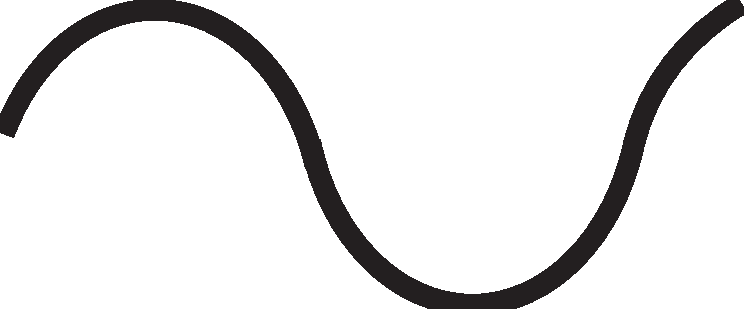
\includegraphics[width=0.05\textwidth]{images/LH035,14,02_115r-d2.pdf}%
%%%%%%%%%%%%%%%%%%%%%%%%%%%%%%%%%%%%%%
~+)
et a rebours s'il retombe d'une même hauteur il aura
tousjours une vitesse\protect\index{Sachverzeichnis}{vitesse} egale.}{\lemma{(3) [...] egale}\Cfootnote{\cite{00311}a.a.O., S. 6f.}}
\pend
\pstart
\edtext{(4)
\textit{Les petits battemens\protect\index{Sachverzeichnis}{battement}}
de \textit{pendule\protect\index{Sachverzeichnis}{pendule}
se font en des temps sensiblement egaux.}}{\lemma{(4) [...] \textit{egaux}}\Cfootnote{\cite{00311}a.a.O., S. 7.}}
\pend
\pstart
\edtext{Prop. 1.\textso{
Probleme.
}\textit{Faire que deux corps se rencontrent avec des vitesses}
ou absolues\protect\index{Sachverzeichnis}{vitesse absolue}
ou respectives\protect\index{Sachverzeichnis}{vitesse respective}
(:~c'est à dire avec lesquelles elles s'approchent ou éloignent~:)
en raison donnée.}{\lemma{Prop. 1. [...] donné}\Cfootnote{\cite{00311}a.a.O., S. 8.}}
\edtext{C'est par le moyen de deux pendules.\protect\index{Sachverzeichnis}{pendule}%
}{\lemma{C'est [...] pendules}\Cfootnote{Siehe \cite{00311}a.a.O., Tafel der Abbildungen, Fig. 3.}}
(+ On le pourroit \edtext{faire
aussi par le moyen}{\lemma{faire}\Bfootnote{%
\textit{(1)}\ par un
\textit{(2)}\ aussi par le moyen
\textit{L}}}
de deux eaux.
Et on auroit en cela l'avantage de les faire choquer aussi obliquement etc.~[+)]\edtext{}{\lemma{+)}\Bfootnote{\textit{erg. Hrsg.}}}
\pend
\pstart
\edtext{Prop. 2.
\textit{Si un corps estant en mouuement est poussé par un autre corps selon la même ligne de direction,
ou selon une autre}[,] \textit{le corps poussé prendra un mouuement qui dependra des deux causes}
[\textit{et sera}]\edtext{}{\lemma{\textit{et sera}}\Bfootnote{\textit{\ erg. Hrsg. nach Vorlage}}}
\textit{composé du premier}
%
[115~v\textsuperscript{o}] %%%%%%%%%% HIER BEGINNT BLATT 115v.
%
\textit{mouuement et du second.}}{\lemma{Prop. 2. [...] \textit{second}}\Cfootnote{\cite{00311}a.a.O., S. 23.}}
\pend
\count\Afootins=1200
\count\Bfootins=1200
\count\Cfootins=1200
%\newpage
\pstart
\edtext{3. prop.\textso{ Principe d'experience.\protect\index{Sachverzeichnis}{experience} }%
\edtext{Si un corps}{\lemma{Si}\Bfootnote{%
\textit{(1)}\ deux corps
\textit{(2)}\ un corps
\textit{L}}}
est meu sur un autre qui est en mouuement,
il \edtext{arrive tout}{\lemma{arrive}\Bfootnote{%
\textit{(1)}\ toute
\textit{(2)}\ tout
\textit{L}}}
ce qui arriveroit si son soustien estoit immobile,
exepté la composition avec le mouuement du soustien.
Il l'enonce autrement
\edtext{mais cela revient}{\lemma{mais}\Bfootnote{%
\textit{(1)}\ il reve
\textit{(2)}\ cela revient
\textit{L}}}
à ce que je dis et par consequent à la proposition precedante.
Il l'enonce à peu près ainsi
que les corps agissent sur eux avec leurs vitesses respectives\protect\index{Sachverzeichnis}{vitesse respective}[,]
quelques puissent estre les propres.%
}{\lemma{3. prop. [...] propres}\Cfootnote{\cite{00311}a.a.O., 25ff.}}
\pend
\pstart
\edtext{\textso{Prop. 4. }%
Principe 3 d'experience.\protect\index{Sachverzeichnis}{experience}
\textit{Si deux corps semblables et}
[\textit{inegaux}]\edtext{}{\lemma{egaux}\Bfootnote{\textit{L ändert Hrsg. nach Vorlage}}}
\textit{de même matiere sont meus avec des vitesses egales}[,]
\edtext{l'effect}{\lemma{l'effect}\Cfootnote{In der Vorlage \textit{l'effort}.}}
\textit{du plus grand corps sera plus grand
que celuy du moindre sur les corps qu'ils rencontreront,
et si deux corps semblables et egaux de même matiere
sont meus avec des vitesses inegales,
celuy qui est meu avec la plus grande vitesse
fera aussi le plus}
\edtext{d'effect\protect\index{Sachverzeichnis}{effet}}{\lemma{d'effect}\Cfootnote{In der Vorlage \textit{d'effort}.}}
\textit{sur les corps qu'il rencontrera,
soit que le choc\protect\index{Sachverzeichnis}{choc} soit horizontal,
ou de bas en haut ou d'autre sorte.}%
}{\lemma{\textso{Prop. 4}. [...] \textit{sorte}}\Cfootnote{\cite{00311}a.a.O., S. 29f.}}
\edtext{Car la plus pesante balle\protect\index{Sachverzeichnis}{balle} jettée fera plus d'effect 
\edtext{que la petite}{\lemma{que la}\Bfootnote{%
\textit{(1)}\ ferré
\textit{(2)}\ petite.
\textit{L}}}.
Et on arrestera plus tost un poutre porté par le courant
\edtext{d'eau, qu'un}{\lemma{d'eau,}\Bfootnote{%
\textit{(1)}\ qu'une
\textit{(2)}\ qu'un
\textit{L}}}
simple baston.}{\lemma{Car [...] baston}\Cfootnote{\cite{00311}a.a.O., S. 30f.}} 
(:~Il y a une autre raison,
par ce qu'on agissant contre le poutre,\protect\index{Sachverzeichnis}{poutre}
on agit contre plus d'eau tout à la fois.
Mais quand on jette [une]\edtext{}{\lemma{un}\Bfootnote{\textit{L ändert Hrsg.}}}
balle\protect\index{Sachverzeichnis}{balle} plus grande, il est assez difficile de dire pourquoy elle fait plus d'effect.\protect\index{Sachverzeichnis}{effet}
Nisi dicendum, idem esse, ut in currente fluminis.
Ut enim plus est in Trabe\protect\index{Sachverzeichnis}{trabis} quod excipit vim fluminis,\protect\index{Sachverzeichnis}{flumen}
quam quod in baculo\protect\index{Sachverzeichnis}{baculum}
unde omnium partium motus.
Sed haec non satis fuerunt.~:)
\pend
\pstart
\edtext{Quantité du Mouuement\protect\index{Sachverzeichnis}{quantité du mouvement} est le produit du corps par la vitesse.\protect\index{Sachverzeichnis}{vitesse}%
}{\lemma{Quantité [...] vitesse}\Cfootnote{\cite{00311}a.a.O., S. 31.}}
\pend
\vspace{1.5em}
\pstart
\noindent
\centering
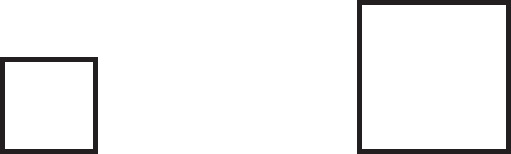
\includegraphics[trim = 0mm -3mm 0mm 0mm, clip, width=0.30\textwidth]{images/LH035,14,02_115v-d0.pdf}\\
\setline{16}\noindent \centering [\textit{Fig. 1}]
\pend
%\newpage
\vspace{1em}
\count\Afootins=1000
\count\Bfootins=1000
\count\Cfootins=1000
\pstart
\edtext{\textso{Prop. 5. Princip. d'exper. 4. }%
\setline{17}\textit{Si un corps en repos suspendu
est choqué horizontalement par un autre corps plus pesant
il resistera moins au mouuement
et le corps chocquant receuura moins d'impression par le choc
que si le corps en repos estoit egalement pesant;
et plus le corps en repos sera pesant
plus il resistera au mouuement}[,]
\textit{pourveu que le corps choquant demeure tousjours le même
et qu'il rencontre tousjours l'autre avec la même vitesse.\protect\index{Sachverzeichnis}{vitesse}}
}{\lemma{\hspace{1.8mm}17-22 \hspace{1.8mm}\textso{Prop. 5}. [...] \textit{vitesse}}\killnumber\Cfootnote{\cite{00311}a.a.O., S. 34.}}
\edtext{La pesanteur\protect\index{Sachverzeichnis}{pesanteur}
ou la tendence vers le centre de gravité\protect\index{Sachverzeichnis}{centre de gravité}
n'en est pas la cause[,]
car le même arrive quand il est chocqué horizontalement.
Item l'air n'en est pas la cause,
car \textit{une boule de plomb de 2 liures resistera plus au mouuement d'une}
[\textit{boule de}]\edtext{}{\lemma{\textit{boule de}}\Bfootnote{\ \textit{erg. Hrsg. nach Vorlage}}}
\textit{terre molle, qu'une boule de bois d'une liure,
quoyque le volume de} la \textit{derniere estant plus grand
elle pousse plus d'air devant soy}
[\textit{et}]\edtext{}{\lemma{\textit{et}}\Bfootnote{\textit{erg. Hrsg. nach Vorlage}}}
\textit{en entraine plus après soy que l'autre.}
La veritable cause de cela[,]
dit il[,]
est la même
qui fait qu'un corps [soit]\edtext{}{\lemma{soit}\Bfootnote{\textit{erg. Hrsg.}}}
plus pesant que l'autre,}{\lemma{La pesanteur [...] l'autre}\Cfootnote{\cite{00311}a.a.O., S. 36f.\hspace{15mm}}}
(+~c'est a dire plus poussé par la cause de la pesanteur:
comme la main jette un solide plus loin qu'un moins solide.
Mons. Des Cartes\protect\index{Namensregister}{\textso{Descartes} (Cartesius, des Cartes), Ren\'{e} 1596-1650}
n'a pas expliqué ny
Mons. de Mariotte\protect\index{Namensregister}{\textso{Mariotte}, Edme (ca.1620-1684)},
ny aucun autre d'où cela peut venir.~[+)]\edtext{}{\lemma{\phantom(\hspace{-1.2mm}+)}\Bfootnote{\textit{erg. Hrsg.}}}
\pend
\pstart
\edtext{\textso{Prop. 6. Principe 5. }%
\textit{Si les quantitez des mouuements\protect\index{Sachverzeichnis}{quantité de mouvement}
de deux corps sont egales lors qu'ils se chocquent directement,
ils s'arresteront l'un l'autre,
et demeureront sans mouuement}
\edtext{(1)}{\lemma{(1)}\Bfootnote{\textit{erg. L}}}%
\edtext{}{\lemma{}\Afootnote{\textit{Am Rand:} (1) $\displaystyle ab\ \sqcap\ ec.$ Ergo $\displaystyle ab - ec\ \sqcap\ 0.$}}
\textit{s'ils s'attachent ensemble,
mais si les deux quantitez de mouuement sont inegales
ils ne demeureront pas en repos immediatement apres le choc.}%
}{\lemma{\textso{Prop. 6}. [...] \textit{choc}}\Cfootnote{\cite{00311}a.a.O., S. 38.}}
Quantité de mouuement\protect\index{Sachverzeichnis}{quantité de mouvement}
est tousjours egale
quand les poids\protect\index{Sachverzeichnis}{poids}
et les vistesses\protect\index{Sachverzeichnis}{vitesse}
sont reciproques.
% \edtext{}{\lemma{Quantité  [...] reciproques}\Cfootnote{\cite{00311}a.a.O., S. 39.}}
\edtext{(2)}{\lemma{(2)}\Bfootnote{\textit{erg. L}}}%
\edtext{}{\lemma{}\Afootnote{\textit{Am Rand:} (2) $\displaystyle \frac{a}{e} \sqcap \frac{c}{b}.$ Ergo $\displaystyle ab\ \sqcap\ ec.$}}
\edtext{Les corps et distances reciproques de statique\protect\index{Sachverzeichnis}{statique}
[ne sont]\edtext{}{\lemma{n'est}\Bfootnote{\textit{L ändert Hrsg.}}}
qu'un cas de ce principe.%
}{\lemma{Les corps  [...] principe}\Cfootnote{\cite{00311}a.a.O., S. 40f.}}
\pend
%\newpage
\vspace{1.5em}
\pstart
%\vspace*{1.0em}% PR: Rein provisorisch !!!
\begin{minipage}[t]{0.50\textwidth}
%\hspace*{-5mm}
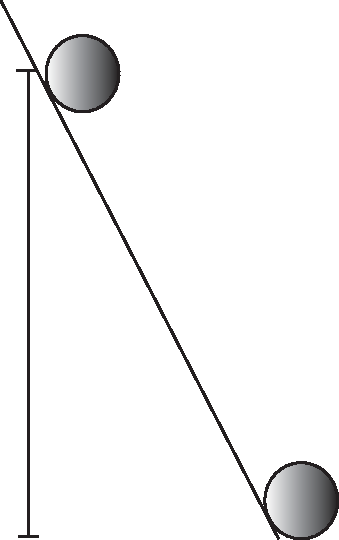
\includegraphics[width=0.35\textwidth]{images/LH035,14,02_115v-d1.pdf}\\
\\
\noindent\centering\hspace*{-17mm}[\textit{Fig. 2}]
\end{minipage}%
\edtext{}{\lemma{}\killnumber\Afootnote{\textit{Am Rand, unter} [\textit{Fig. 2}]:
NB. Examinandum.\vspace{-8mm}}}
\hspace{5mm}
\begin{minipage}[t]{0.50\textwidth}
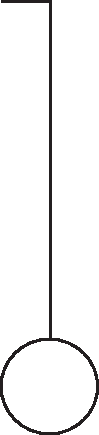
\includegraphics[width=0.17\textwidth]{images/LH035,14,02_115v-d4.pdf}\\
\\
\noindent\centering\hspace*{-17mm}[\textit{Fig. 3}]
% \vspace{1em}
\end{minipage}
\pend
\newpage
%\vspace{1.5em}
\count\Afootins=1100
\count\Bfootins=1100
\count\Cfootins=1100
\pstart
\edtext{\textso{Prop. 7. }%
\textit{Si deux corps inegaux en pesanteur\protect\index{Sachverzeichnis}{pesanteur}
sont meus avec des vitesses\protect\index{Sachverzeichnis}{vitesse} egales}
[\textit{leurs}]\edtext{}{\lemma{leur}\Bfootnote{\textit{L ändert Hrsg. nach Vorlage}}}
\textit{quantités de mouuement\protect\index{Sachverzeichnis}{quantité de mouvement}
seront l'une à l'autre en la raison de leurs poids.\protect\index{Sachverzeichnis}{poids}}%
}{\lemma{\textso{Prop. 7}. [...] \textit{poids}}\Cfootnote{\cite{00311}a.a.O., S. 45.}}
\edtext{(3)}{\lemma{(3)}\Bfootnote{\textit{erg. L}}}%
\edtext{}{\lemma{}\Afootnote{\textit{Am Rand:} (3) $\displaystyle \frac{ab}{eb} \sqcap \frac{a}{e}.$\vspace{2mm}}}
\pend
\pstart
\edtext{\textso{Prop. 8. }%
De même
\textit{si deux corps egaux en pesanteur\protect\index{Sachverzeichnis}{pesanteur}
sont meus avec des vitesses inegales}
[\textit{leurs}]\edtext{}{\lemma{leur}\Bfootnote{\textit{L ändert Hrsg. nach Vorlage}}}
\textit{quantités de mouuement seront entre elles comme}
[\textit{leurs}]\edtext{}{\lemma{leur}\Bfootnote{\textit{L ändert Hrsg. nach Vorlage}}}
\textit{vitesses.}%
}{\lemma{\textso{Prop. 8}. [...] \textit{vitesses}}\Cfootnote{\cite{00311}a.a.O., S. 46.\hspace{15mm}}}
\edtext{(4)}{\lemma{(4)}\Bfootnote{\textit{erg. L}}}%
\edtext{}{\lemma{}\Afootnote{\textit{Am Rand:} (4) $\displaystyle \frac{ab}{ac} \sqcap \frac{b}{c}.$\vspace{2mm}}}
\pend
\pstart
\edtext{\textso{Prop. 9. }%
\textit{Si deux corps ont}
[\textit{leurs}]\edtext{}{\lemma{leur}\Bfootnote{\textit{L ändert Hrsg. nach Vorlage}}}
\textit{poids et}
[\textit{leurs}]\edtext{}{\lemma{leur}\Bfootnote{\textit{L ändert Hrsg. nach Vorlage}}}
\textit{vitesses inegales}
[\textit{leurs}]\edtext{}{\lemma{leur}\Bfootnote{\textit{L ändert Hrsg. nach Vorlage}}}
\textit{quantitez de mouuement seront l'une à l'autre en la raison composée des poids et des vitesses.}%
}{\lemma{\textso{Prop. 9}. [...] \textit{vitesses}}\Cfootnote{\cite{00311}a.a.O., S. 47.}}
\edtext{(5)}{\lemma{(5)}\Bfootnote{\textit{erg. L}}}%
\edtext{}{\lemma{}\Afootnote{\textit{Am Rand:} (5) $\displaystyle \frac{ab}{ec} \sqcap \frac{a}{e} \smallfrown \frac{b}{c}.$\vspace{2mm}}}
\pend
\pstart
\edtext{\textso{Prop. 10. }%
ou 6\textsuperscript{me} principe d'experience:
\textit{Si un corps mol sans}
\edtext{\textit{ressort} a chocqué%
}{\lemma{\textit{ressort}}\Bfootnote{%
\textit{(1)}\ \textit{chocque}
\textit{(2)}\ a chocqué
\textit{L}}}
\textit{directement un autre corps mol\protect\index{Sachverzeichnis}{corps mol}
et sans ressort\protect\index{Sachverzeichnis}{ressort},
les deux ensemble estant joints après le choc,\protect\index{Sachverzeichnis}{choc}
iront de même part que le corps chocquant,
et la quantité de mouuement des deux ensemble sera egale
à la quantité de mouuement\protect\index{Sachverzeichnis}{quantité de mouvement}}
[\textit{de ce corps}]\edtext{}{\lemma{\textit{de ce corps}}\Bfootnote{\ \textit{erg. Hrsg. nach Vorlage}}}
\textit{avant le chocq.}%
}{\lemma{\textso{Prop. 10}. [...] \textit{chocq}}\Cfootnote{\cite{00311}a.a.O., S. 48f.\hspace{15mm}}}
\edtext{(6)}{\lemma{(6)}\Bfootnote{\textit{erg. L}}}%
\edtext{}{\lemma{}\Afootnote{\hspace{-1.8mm}\textit{Am Rand:} (6) $\displaystyle ab\ \!\pPsMs\, e0 \, \sqcap\, ab.$}}
Donc \edtext{\textit{pour trouver quelle doit estre la vitesse\protect\index{Sachverzeichnis}{vitesse}}
de \textit{deux corps mols joints après
\edtext{le chocq, il faut}{\lemma{}\Bfootnote{\textit{le chocq,}\ \textbar\ se avoir \textit{streicht Hrsg.}\ \textbar\ \textit{il faut}}}
diviser la premiere quantité de mouuement}
du corps chocquant\protect\index{Sachverzeichnis}{corps choquant}
par la somme des corps, le quotient sera la vitesse de la somme.%
}{\lemma{\textit{pour}
 [...] somme}\Cfootnote{\cite{00311}a.a.O., S. 52. Zitat mit Auslassung.}}
\edtext{(7)}{\lemma{(7)}\Bfootnote{\textit{erg. L}}}%
\edtext{}{\lemma{}\Afootnote{\hspace{-1.8mm}\textit{Am Rand:} (7) $\displaystyle\frac{ab}{a +e}.$\vspace{-8mm}}} 
\pend
\count\Afootins=1200
\count\Bfootins=1200
\count\Cfootins=1200
\pstart
\edtext{\textso{Prop. 11. Princip. de exp. 7. }%
\textit{Si deux corps mols\protect\index{Sachverzeichnis}{corps mol}
sans ressort\protect\index{Sachverzeichnis}{ressort}
vont de même part avec des vistesses inegales
et que le plus viste rencontre l'autre directement,
ils auront ensemble après qu'ils seront joints
une quantité de mouuement\protect\index{Sachverzeichnis}{quantité de mouvement}
egale à la somme des quantitez de mouuement des deux corps avant le chocq.}%
}{\lemma{\textso{Prop. 11}. [...] \textit{chocq}}\Cfootnote{\cite{00311}a.a.O., S. 56f.}}
\edtext{(8)}{\lemma{(8)}\Bfootnote{\textit{erg. L}}}%
\edtext{}{\lemma{}\Afootnote{\textit{Am Rand:} (8) $\displaystyle ab + ec \, \sqcap \, ab + ec.$%
\ \ $\displaystyle a + e, \smallfrown f.$}} 
\pend
\pstart
\edtext{\textso{Prop. 12. princip. d'Exp. 8. }%
\textit{Si deux corps mols\protect\index{Sachverzeichnis}{corps mol}
sans ressort\protect\index{Sachverzeichnis}{ressort}
egaux ou inegaux se rencontrent directement,
allant l'un contre l'autre avec des vitesses egales ou inegales,
et que leurs quantités de mouuement\protect\index{Sachverzeichnis}{quantité de mouvement}
soient inegales avant de chocq,
la moindre quantité de mouuement se perdra entierement,
et il s'en perdra autant de l'autre,
et les deux corps joints ensemble n'auront plus que la}
\edtext{vitesse}{\lemma{vitesse}\Cfootnote{In der Vorlage \textit{quantité de movement}.}}
\textit{restante, c'est à dire la difference des deux quantitez de mouuement avant le chocq,
et cette difference divisée par la somme des poids
donnera la vitesse\protect\index{Sachverzeichnis}{vitesse} commune
des deux corps joints aprés le chocq.\protect\index{Sachverzeichnis}{choc}}%
}{\lemma{\textso{Prop. 12}. [...] \textit{chocq}}\Cfootnote{\cite{00311}a.a.O., S. 60f.}}
\edtext{(9)}{\lemma{(9)}\Bfootnote{\textit{erg. L}}}%
\edtext{}{\lemma{}\Afootnote{\textit{Am Rand:} (9) $\displaystyle \pPsMs\, ab\ \pMsPs\, ec \ \sqcap \ \pPsMs\, ab\ \pMsPs\, ec.$%
\ \ $\displaystyle (a + e, \smallfrown f)$ $\displaystyle \text{et}\ f \, \sqcap\, \frac{\PsPsMs\! \efrac{\efrac{}{\efrac{\displaystyle ab}{}}}{}\ \PsMsPs\! \efrac{\efrac{}{\efrac{\displaystyle ec}{}}}{}}{a + e}.$\vspace{2mm}}}
\pend
%\newpage
\pstart
\edtext{\textso{Prop. 13. }\edtext{%
\textit{Si}}{%
\lemma{\textso{Prop. 13.}}\Bfootnote{%
\textit{(1)}\ Soit
\textit{(2)}\ \textit{Si}
\textit{L}}}
\textit{une ligne comme $\displaystyle AB$
\edtext{est}{\lemma{est}\Bfootnote{\ \textit{erg. L}}}
divisée au point $\displaystyle C$
en raison reciproque des poids\protect\index{Sachverzeichnis}{poids}
des corps $\displaystyle A$ et $\displaystyle B$
et \edtext{qu'estant prolongée}{\lemma{qu'estant}\Bfootnote{%
\textit{(1)}\ rencontrée
\textit{(2)}\ \textit{prolongée}
\textit{L}}}
directement de part et d'autre}[,]
\textit{on y prenne un point $\displaystyle D$
en sorte qu'$\displaystyle AD$ represente la vitesse\protect\index{Sachverzeichnis}{vitesse}
et la direction\protect\index{Sachverzeichnis}{direction} du corps $\displaystyle A$
avant le chocq,\protect\index{Sachverzeichnis}{choc}
et $\displaystyle BD$ celle du corps $\displaystyle B$,
l'une et l'autre vitesse} estant \textit{supposée
\edtext{uniforme,
et que $\displaystyle DE$ soit prise egale à $\displaystyle CD$,
les deux corps}{\lemma{uniforme,}\Bfootnote{%
\textit{(1)}\ \textit{et que deux corps}
\textit{(2)}\ \textit{et que} [...] \textit{corps}
\textit{L}}}
\edtext{s'estant joints ensemble iront avec}{\lemma{s'estant}\Bfootnote{%
\textit{(1)}\ \textit{joints iront}
\textit{(2)}\ \textit{joints ensemble iront}
\textit{(a)}\ de
\textit{(b)}\ \textit{avec}
\textit{L}}}
la vitesse et la direction} de la ligne \textit{$\displaystyle DE,$
s'ils sont sans ressort.\protect\index{Sachverzeichnis}{ressort}}}{%
\lemma{\textso{Prop. 13}. [...] \textit{ressort}}\Cfootnote{\cite{00311}a.a.O., S. 68. Zitat mit Auslassung.}}
(+~Ut bene enuntietur propositio intelligendum $\displaystyle DE,$ sumi in partes aversas a $\displaystyle C.$~+)
Il ne demonstre pas universellement cette proposition
quoyque cela se puisse,
mais il ne la prouue que par l'induction\protect\index{Sachverzeichnis}{induction} des precedantes.
\edtext{(10)}{\lemma{(10)}\Bfootnote{\textit{erg. L}}}%
\edtext{}{\lemma{}\Afootnote{\textit{Am Rand:} (10) $\displaystyle f \, \sqcap\, DE.$
Directio\textsuperscript{[a]} ejus corporis celeritatem\protect\index{Sachverzeichnis}{celeritas} sequitur,
cujus signum in ipsius $\displaystyle f$ valore praevalet,
fere ut in Methodo tangentium.\textsuperscript{[b]}\protect\label{LH035,14,02_115v-ref1}%
\vspace{2mm}\\
\footnotesize
\textsuperscript{[a]} %
Directio %
\textit{(1)}\ in ea %
\textit{(2)}\ \textbar\ in \textit{streicht Hrsg.}\ \textbar\ ejus %
\textit{L}
\quad %
\textsuperscript{[b]} %
Methodo tangentium: Siehe etwa \textit{LSB} VII, 5 N.~7, 8, 9, 10 und 14. \cite{01063}\vspace{-6mm}}}
\pend
\newpage
\pstart
%\vspace*{2em}
\noindent
\centering
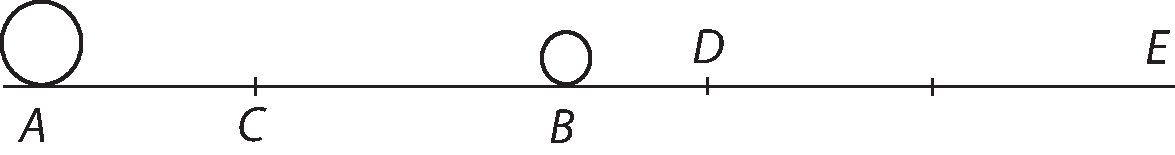
\includegraphics[trim = 0mm -3mm 0mm 0mm, clip, width=0.65\textwidth]{images/LH035,14,02_115v-d2.pdf}\\
\noindent \centering [\textit{Fig. 4}]\edtext{}{\lemma{\hspace{1.8mm}[\textit{Fig. 4}]}\killnumber\Cfootnote{\cite{00311}Siehe a.a.O., Tafel der Abbildungen, Fig. 7.}}%
\pend
\vspace{2em}
\pstart
\edtext{\textso{Prop. 14. }%
\setline{1}Huitieme
(jam adfuit debebat dici 9\textsuperscript{me})
principe de experience.
\textit{Si un corps inébranslable à ressort a changé sa figure
et s'est mis en ressort\protect\index{Sachverzeichnis}{ressort} par le choc d'un corps dur}[,]
\textit{en se restituant et reprenant sa premiere figure,
il redonnera à ce corps la même vitesse\protect\index{Sachverzeichnis}{vitesse}
qu'il avoit immediatement avant le choc.\protect\index{Sachverzeichnis}{choc}}%
}{\lemma{1-4 \hspace{1.8mm}\textso{Prop. 14}. [...] \textit{choc}}\killnumber\Cfootnote{\cite{00311}a.a.O., S. 73.}}
\pend
\count\Afootins=1000
\count\Bfootins=1200
\count\Cfootins=1200
%\newpage
\pstart
\edtext{\textso{Prop. 15. }%
\textit{Si deux corps à ressort\protect\index{Sachverzeichnis}{ressort}
se chocquent directement avec des vitesses reciproques à leurs poids,\protect\index{Sachverzeichnis}{poids}
chacun de ces corps retournera en arriere avec sa premiere vitesse.\protect\index{Sachverzeichnis}{vitesse}}%
}{\lemma{\textso{Prop. 15}. [...] \textit{vitesse}}\Cfootnote{\cite{00311}a.a.O., S. 90.}}%
\edtext{}{\lemma{}\Afootnote{\textit{Am Rand:}
Demonstratio prop. 15 huc redit apud autorem,
quod\textsuperscript{[a]} duo corpora Elaterii aequalis celeritatum\protect\index{Sachverzeichnis}{celeritas}
ponderibus\protect\index{Sachverzeichnis}{pondus} reciprocarum
ictu\protect\index{Sachverzeichnis}{ictus} perdunt motum concursus;
et idem evenit ac si quodlibet eorum ostendisset corpus immobile et [inflexibile]\textsuperscript{[b]}
quo casu sua celeritate rediret.
(+~Hoc demonstrandum,
idem evenire, quod autor non facit,
idem inquam evenire, ac si singula ostendere
intelligerentur corpus durum inflexile.~[+\phantom(\hspace{-1.2mm})]\textsuperscript{[c]}\vspace{2mm}\\
\footnotesize
\textsuperscript{[a]} %
quod %
\textit{(1)}\ duobus %
\textit{(2)}\ duo %
\textit{L}
\quad %
\textsuperscript{[b]} %
inflexible %
\textit{L ändert Hrsg.}
\quad %
\textsuperscript{[c]} %
+\phantom(\hspace{-1.2mm}) \textit{erg. Hrsg.}\vspace{-4mm}}}%
\pend
\pstart
\edtext{\textso{Consequence. }%
Il s'ensuit
\textit{que deux corps egaux ou inegaux estant pressez l'un contre l'autre,
et mis en ressort, par quelque cause que ce soit,
si la pression cesse tout à coup,
ils se repousseront l'un l'autre par}
[\textit{leurs}]\edtext{}{\lemma{leur}\Bfootnote{\ \textit{L ändert Hrsg. nach Vorlage}}}
\textit{ressorts et en se repoussant chacun} entre \textit{eux
prendra une egale \protect\index{Sachverzeichnis}{quantité de mouvement}quantité de}
\edtext{\textit{mouuement}\edtext{\textit{.} Ce qui}{% ?????
\lemma{}\Bfootnote{\textit{mouuement.}\ \textbar\ Car leur forcer \textit{streicht Hrsg.}\ \textbar\ Ce qui\ \textit{L}}}}{%
\lemma{Zur Variante \textit{mouuement.} Ce qui}%
\Cfootnote{\textit{forcer} ist abbrechendes Wort, möglicherweise für \textit{forcement}.}}
est toute la même chose
comme si nous nous imaginions deux corps qui perdroient
[leurs]\edtext{}{\lemma{leur}\Bfootnote{\ \textit{L ändert Hrsg.}}}
vistesses\protect\index{Sachverzeichnis}{vitesse}
s'ils estoient sans ressort,\protect\index{Sachverzeichnis}{ressort}
d'où vient qu'aprés le choc\protect\index{Sachverzeichnis}{choc}
le ressort les separant fera tout autant qu'il fait en separant ceux
qui sont venu avec des vitesses reciproques aux poids.\protect\index{Sachverzeichnis}{poids}
C'est à dire il donnera à chacun sa premiere vitesse,
et par consequent la même quantité de mouuement,
donc il donnera aussi la même quantité de mouuement
à deux balles\protect\index{Sachverzeichnis}{balle} pressées simplement l'une contre
\edlabel{35,14,02_115v_01}%%%%
\edtext{l'autre.}{{\xxref{35,14,02_115v_01}{35,14,02_115v_02}}\lemma{l'autre.}\Bfootnote{%
\textit{(1)}\ \textit{Il s'ensuit aussi, que deux corps à ressort qui se sont rencontrez directement partagent par le mouuement de ressort la vitesse respective de leur choc.}
\textit{(2)}\ Cette consequence [...] principe car
\textit{(a)}\ puisque
\textit{(b)}\ : ils resisteront [...] \textit{leur choc.}
\textit{L}}}
Cette consequence aussi se peut juger veritable par un autre principe
car: ils resisteront au ressort\protect\index{Sachverzeichnis}{ressort}
qui les separe en raison de leurs poids,
et par consequent la quantité de mouuement\protect\index{Sachverzeichnis}{quantité de mouvement}
sera la même.}{\lemma{\textso{Consequence} [...] la même}\Cfootnote{\cite{00311}a.a.O., S. 94f.}}
\edtext{Mons. de Mariotte\protect\index{Namensregister}{\textso{Mariotte}, Edme, Seigneur de Chazeuil ca. 1620-1684}
juge cette consequence probable simplement,}{\lemma{Mons. [...] simplement}\Cfootnote{\cite{00311}a.a.O., S. 95.}}
mais elle me semble aussi demonstrative que l'autre;
et même estre le principe
[direct]\edtext{}{\lemma{}\Bfootnote{directe \textit{L ändert Hrsg.}}}
pour demonstrer l'autre.
\pend
\vspace{1em}
\pstart
%
\noindent
\centering
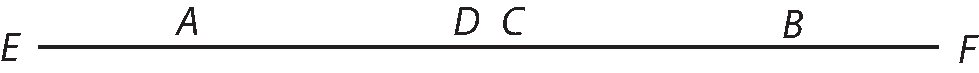
\includegraphics[trim = 0mm -3mm 0mm 0mm, clip, width=0.7\textwidth]{images/LH035,14,02_115v-d3.pdf}\\
\noindent \centering [\textit{Fig. 5}]\edtext{}{\lemma{\hspace{1.5mm}[\textit{Fig. 5}]}\killnumber\Cfootnote{\cite{00311}Siehe a.a.O., Tafel der Abbildungen, Fig. 11.}}%
\pend
\vspace{1em}% PR: Rein provisorisch !!!
%%%%%%%%%%%%%%%%%%%% 
\pstart
\edtext{2\textsuperscript{de} consequence.}{\lemma{\hspace{1.8mm}6-S.428.14 \hspace{1.8mm}2\textsuperscript{de} consequence [...] en repos}\killnumber\Cfootnote{\cite{00311}a.a.O., S. 96f. Zweites Zitat mit Auslassungen.}}\setline{6}
\textit{Il s'ensuit aussi, que deux corps à ressort
qui se sont recontrez directement,\hfill
partagent\hfill par\hfill le\hfill mouuement\hfill de\hfill ressort\protect\index{Sachverzeichnis}{ressort}\hfill
la\hfill vitesse\hfill respective\hfill de\hfill leur\hfill chocq.}%
\edlabel{35,14,02_115v_02}%%%%
%%%%
\edtext{}{\lemma{}\Afootnote{\textit{Am Rand:} %
\textsuperscript{[a]}Celeritas respectiva\protect\index{Sachverzeichnis}{celeritas respectiva}
$\displaystyle d\ \sqcap\ \pPsPsMs b\ \pPsMsPs c$
est scilicet aut summa aut differentia\textsuperscript{[b]}
celeritatum absolutarum.
Hoc non satis autori observatum.%
\protect\index{Sachverzeichnis}{vis elaterii}\textso{ Vis Elaterii} est\textsuperscript{[c]}
$\displaystyle \pMsPsMs ab\ \pMsMsPs ec.$
Igitur cum\textsuperscript{[d]}
celeritas respectiva\protect\index{Sachverzeichnis}{celeritas respectiva}
aut quantitas motus\protect\index{Sachverzeichnis}{quantitas motus} significant summam,
vis Elaterii\protect\index{Sachverzeichnis}{vis elaterii} differentiam significabit et contra.
Haec vis separatrix in duas partes secanda est,
et erit $\protect\displaystyle gl + g \frac{al}{e}\ \sqcap\ \pMsPsMs ab\ \pMsMsPs ec$
unde $\protect\displaystyle g\, \sqcap \frac{\MsPsMs\! \efrac{\efrac{}{\efrac{\displaystyle aeb}{}}}{} \MsMsPs\! \efrac{\efrac{}{\efrac{\displaystyle e^2c}{}}}{}}{al + el}$
et celeritas corporis $\displaystyle a$
orta a reflexione seu $\displaystyle \beta$
erit: $\protect\displaystyle \beta\, \sqcap\, g\ \sqcap\ \pMsPsMs aeb\ \pMsMsPs e^2c, \smallsmile al + el$
et celeritas corporis $\displaystyle e$
post reflexum seu $\displaystyle \gamma$
erit $\protect\displaystyle \sqcap \frac{\MsPsMs\! \efrac{\efrac{}{\efrac{\displaystyle a\cancel{e}b}{}}}{} \MsMsPs\! \efrac{\efrac{}{\efrac{\displaystyle e^{\cancel{2}}ac}{}}}{}}{a\cancel{e}l + e^{\cancel{2}}l}$
ponendo $\displaystyle l \ \sqcap\ 1.$%
\vspace{2mm}\\
\footnotesize
\textsuperscript{[a]} %
\textit{(1)}\ Vis respectiva, $\displaystyle d\ \sqcap$\ %
\textit{(2)}\ Vis\ %
\textit{(3)}\ Celeritas respectiva\ %
\textit{L}
\quad %
\textsuperscript{[b]} %
differentia %
\textit{(1)}\ quantitatum\ %
\textit{(2)}\ celeritatum\ %
\textit{L}
\quad %
\textsuperscript{[c]} %
est %
\textit{(1)}\ $\displaystyle \pPsPsMs ab\ \pPsMsPs ec$\ %
\textit{(2)}\ $\displaystyle \pPsMsPs ab\ \pPsPsMs ec$\ %
\textit{(3)}\ $\displaystyle \pMsPsMs ab\ \pPsPsMs ec$\ %
\textit{(4)}\ $\displaystyle \pMsPsMs ab\ \pMsMsPs ec$\ %
\textit{L} 
\quad %
\textsuperscript{[d]}%
cum %
\textit{(1)}\ vis\ %
\textit{(2)}\ celeritas\ %
\textit{L}%
\vspace{-4mm}% PR: Rein provisorisch.
}}
%%%%
\pend
\count\Afootins=1200
\count\Bfootins=1200
\count\Cfootins=1200
\newpage
\pstart \noindent Car par la definition de la vitesse respective,\protect\index{Sachverzeichnis}{vitesse respective}
c'est à dire avec la quelle deux corps s'approchent ou s'eloignent,
si deux corps se rencontrent dans le point $\displaystyle C$ de la ligne $\displaystyle AB,$
avec les vitesses $\displaystyle AC.$ $\displaystyle BC,$
ou dans le point $\displaystyle D$ ou $\displaystyle E$
\edtext{ou $\displaystyle F$}{\lemma{ou $\displaystyle F$}\Bfootnote{\ \textit{erg. L}}}
de la même ligne,
\edtext{avec la vitesse}{\lemma{avec}\Bfootnote{%
\textit{(1)}\ le point
\textit{(2)}\ la vitesse
\textit{L}}}
$\displaystyle AD$ et $\displaystyle BD,$
[leurs]\edtext{}{\lemma{leur}\Bfootnote{\textit{L ändert Hrsg.}}}
vitesses respectives\protect\index{Sachverzeichnis}{vitesse respective} seront tousjours les mêmes.
Or, \textit{par la troisiesme proposition, l'impression}
\edtext{\textit{du ressort} (puto agendum du choc) \textit{qu'elles feront l'une}}{\lemma{\textit{du}}\Bfootnote{%
\textit{(1)}\ chocq, \textit{qu'elles feront l'une}
\textit{(2)}\ \textit{ressort} [...] \textit{l'une}
\textit{L}}}
\textit{sur l'autre sera la même,
et par consequent elles prendront une force de ressort\protect\index{Sachverzeichnis}{ressort}
aussi promte et aussi ferme} que
\textit{quand elles se rencontrent en $\displaystyle C.$}
Mais en $\displaystyle C$ elles partageront
\textit{leur vitesse respective $\displaystyle AB,$
selon la proportion reciproque de leurs poids,\protect\index{Sachverzeichnis}{poids}
puisque la} \protect\index{Sachverzeichnis}{boule}[\textit{boule}]\edtext{}{\lemma{boulle}\Bfootnote{\ \textit{L ändert Hrsg. nach Vorlage}}}
\textit{$\displaystyle A$ prend la vitesse $\displaystyle AC,$
et $\displaystyle B$ la vitesse $\displaystyle BC,$}
[\textit{donc}]\edtext{}{\lemma{dont}\Bfootnote{\ \textit{L ändert Hrsg. nach Vorlage}}}
\textit{au point $\displaystyle D$ elles partageront de même leur vitesse respective.}\protect\index{Sachverzeichnis}{vitesse respective}
Car la vitesse respective est representée par toute la ligne $\displaystyle AB$
dont les partages [se]\edtext{}{\lemma{se}\Bfootnote{\textit{erg. Hrsg.}}}
feront tousjours de même en raison des poids,
sans avoir égard aux raisons des vitesses du \protect\index{Sachverzeichnis}{concours}concours.%
\edtext{}{\lemma{}\Afootnote{\textit{Am Rand:} Belle observation que les reflexions sont independantes des vitesses absolues du concours.\protect\index{Sachverzeichnis}{concours}\vspace{-6mm}}}
Le même arrivera si au lieu du point $\displaystyle D$ ou $\displaystyle C$
\edtext{nous prennions}{\lemma{nous}\Bfootnote{%
\textit{(1)}\ prendrions
\textit{(2)}\ prennions
\textit{L}}}
un autre $\displaystyle E$ ou $\displaystyle F,$
hors de la \edtext{ligne
quand}{\lemma{ligne}\Bfootnote{%
\textit{(1)}\ . Ou dans
\textit{(2)}\ quand
\textit{L}}}
[tous]\edtext{}{\lemma{toux}\Bfootnote{\textit{L ändert Hrsg.}}}
deux vont de même sens,
ou dans les points $\displaystyle A.$ $\displaystyle B$
quand un est en repos.
%
[112~r\textsuperscript{o}]%%%%%%%%%% HIER BEGINNT BLATT 112r (Nachfolger von Blatt 115v).
%
\pend
\pstart
Diximus corpora Elatere\protect\index{Sachverzeichnis}{elater} praedita[,]
\edtext{si talia sint ut sine Elatere quiescerent[,]}{\lemma{si talia [...] quiescerent}\Bfootnote{\textit{erg. L}}}
post concursum\protect\index{Sachverzeichnis}{concursus}
celeritatem respectivam\protect\index{Sachverzeichnis}{celeritas respectiva}
dividere in duas absolutas in reciproca corporum ratione;
per reflexionem.
Nec referre quae corporum \edtext{concurrentium
celeritas}{\lemma{concurrentium}\Bfootnote{%
\textit{(1)}\ vis\protect\index{Sachverzeichnis}{vis}
\textit{(2)}\ celeritas
\textit{L}}}
absoluta fuerit.
Cum celeritas respectiva sit quae ictus\protect\index{Sachverzeichnis}{ictus} magnitudinem \edtext{facit\edtext{.
Eaque occasione recte dixit
Mariottus\protect\index{Namensregister}{\textso{Mariotte}, Edme, Seigneur de Chazeuil ca. 1620-1684}
idem cogitandum de corporibus}{\lemma{facit.}\Bfootnote{%
\textit{(1)}\ Sed hactenus locuti sumus de corpori
\textit{(2)}\ Eaque [...] corporibus
\textit{L}}}
quibuslibet quae Elaterium quoddam a se invicem separare conatur,
ut si pila quadam oneres exiguum
[Tubum]\edtext{}{\lemma{Tubuum}\Bfootnote{\textit{L ändert Hrsg.}}}
octupli ponderis\protect\index{Sachverzeichnis}{pondus},
octuplo tardius recedet Tormentum quam procedit pila.\protect\index{Sachverzeichnis}{pila}
Sed \edtext{et si nulla adsit pila\protect\index{Sachverzeichnis}{pila},}{\lemma{et si}\Bfootnote{%
\textit{(1)}\ nullus adsit canon,
\textit{(2)}\ nulla adsit pila,
\textit{L}}}
aer ipse nonnihil dilataturae se flammae\protect\index{Sachverzeichnis}{flamma} resistet,
tum quia corpus ut aer\protect\index{Sachverzeichnis}{aer}
remis,\protect\index{Sachverzeichnis}{remus} tum quia Elasticus.
De même dit il, la flamme\protect\index{Sachverzeichnis}{flamme}
d'une fusée\protect\index{Sachverzeichnis}{fusée} \textit{choquant l'air}
en [avant]\edtext{}{\lemma{arriere}\Bfootnote{\textit{L ändert Hrsg.}}}
\textit{avec impetuosité donne un mouuement en arrière au corps de la fusée,
et si l'on suspend un vaisseau cylindrique plein d'eau,
où l'on ait ajusté un peu plus haut que la base un petit tuyau oblique,
l'eau qui jaillira par ce petit tuyau
donnera un mouuement circulaire assez viste
à ce vaisseau\protect\index{Sachverzeichnis}{vaisseau}
par le choc de l'air\protect\index{Sachverzeichnis}{air}}
(+~NB. mensurari hac ratione forte possit quantitas resistentiae aeris\protect\index{Sachverzeichnis}{resistentia aeris}~+),
\textit{ou par le choc\protect\index{Sachverzeichnis}{choc} de l'eau\protect\index{Sachverzeichnis}{eau}
si on le met dans un vaisseau plein d'eau sans qu'il touche au}
\edtext{fonds.}{\lemma{fonds}\Cfootnote{In der Vorlage \textit{fond}.}}%
}{\lemma{Eaque [...] fonds}\Cfootnote{\cite{00311}a.a.O., S. 98-100.}}
(+~NB. cela peut servir à mesurer les differences des resistences de l'air et de l'eau.\protect\index{Sachverzeichnis}{resistentia aquae}~[+)]\edtext{}{\lemma{+}\Bfootnote{\textit{erg. Hrsg.}}}
\pend
\count\Afootins=1200
\count\Bfootins=1000
\count\Cfootins=1000
\pstart
\edtext{\textso{Prop. 16. }%
\textit{Si deux corps à ressort\protect\index{Sachverzeichnis}{ressort} sont egaux
et que l'un chocque directement l'autre en repos,
ce dernier prendra la vitesse\protect\index{Sachverzeichnis}{vitesse} entiere de l'autre après le chocq,\protect\index{Sachverzeichnis}{choc}
et le fera rester sans mouuement}}{\lemma{\textso{Prop. 16}. [...] \textit{mouuement}}\Cfootnote{\cite{00311}a.a.O., S. 100.\hspace{15mm}}}
(+~das findet sich im spiel der birckentafeln~+).
%
\edtext{Consequence. Si celuy qui est choqué
est \textit{moindre en poids\protect\index{Sachverzeichnis}{poids}
ils s'avanceront tous deux après le chocq
et} s'il \textit{est plus pesant,
le corps chocquant retournera en arriere.}}{\lemma{Consequence [...] \textit{en arriere}}\Cfootnote{\cite{00311}a.a.O., S. 102f. Zitat mit Auslassungen.\hspace{35mm}}}
%
\edtext{L'applatissement dans les corps à ressorts se fait de même que dans les corps
\edtext{mols, mais}{\lemma{mols,}\Bfootnote{%
\textit{(1)}\ seulement
\textit{(2)}\ mais
\textit{L}}}
[ils]\edtext{}{\lemma{elles}\Bfootnote{\textit{L ändert Hrsg.}}}
se restituent.
\textit{Les corps qui ont un ressort lent comme les ballons,\protect\index{Sachverzeichnis}{ballon}}
(:~s\c{c}avoir \edtext{dont l'applatissement et la restitution sont sensibles}{\lemma{dont}\Bfootnote{%
\textit{(1)}\ la restitution est visi
\textit{(2)}\ l'applatissement et la restitution
\textit{(a)}\ se font
\textit{(b)}\ sont sensibles
\textit{L}}}~:)
\textit{s'avancent un peu par le mouuement simple pendant}
l'applatissement et la restitution.}{\lemma{L'applatissement [...] restitution}\Cfootnote{\cite{00311}a.a.O., S. 103-105.}}
%
\edtext{Si une boule\protect\index{Sachverzeichnis}{boule} à ressort roule sur un plan,
et choque une autre directement en
\edtext{repos du même poids et}{\lemma{repos}\Bfootnote{
\textit{(1)}\ d'un poids et
\textit{(2)}\ du même poids et
\textit{L}}}
matiere\protect\index{Sachverzeichnis}{matière}
\textit{elle ne perdra pas tout son mouuement}[,]
\textit{comme on le voit par l'experience dans les jeux de billard.\protect\index{Sachverzeichnis}{billard}
Ce qui procede de ce qu'elle ne donne à l'autre boule que sa vitesse directe,
% S. 105f.
mais pas son mouuement en rond,}
qu'elle \textit{conserve, ce qui la fait encore rouler et suivre l'autre,
% S. 106.
mais avec beaucoup moins de vitesse;\protect\index{Sachverzeichnis}{vitesse}}
le même \textit{arrivera quoyque la boule qui chocque ne roule pas,
si les deux boules\protect\index{Sachverzeichnis}{boule} ont un ressort\protect\index{Sachverzeichnis}{ressort} imparfait;}
comme si elles sont de bois.
}{\lemma{Si une [...] de bois}\Cfootnote{\cite{00311}a.a.O., S.~105f. Zitat mit Auslassungen.}}
\pend
\pstart
%
\edtext{\textso{Prop. 17. }%
\textit{Si deux boules à ressort égales se choquent avec des vitesses\protect\index{Sachverzeichnis}{vitesse}
inegales elles feront echange de}
[\textit{leurs}]\edtext{}{\lemma{leur}\Bfootnote{\textit{L ändert Hrsg. nach Vorlage}}}
\textit{vitesses.}%
}{\lemma{\textso{Prop. 17}. [...] \textit{vitesses}}\Cfootnote{\cite{00311}a.a.O., S. 107.\hspace{15mm}}}
Cela se demonstre par la simple composition de deux
\edtext{mouuements[:] le reste du mouuement
simple, en les considerant comme corps sans ressorts;\protect\index{Sachverzeichnis}{ressort}
et celuy du ressort.}{\lemma{mouuements[:]}\Bfootnote{%
\textit{(1)}\ celuy du ressort, et celuy
\textit{(2)}\ . Celuy
\textit{(3)}\  le reste [...]  du ressort.
\textit{L}}}
%
Car \edtext{\textit{soyent deux Boules\protect\index{Sachverzeichnis}{boule}
egales \edtext{à ressort $\displaystyle A$ et $\displaystyle B,$}{\lemma{\protect{à} ressort}\Bfootnote{%
\textit{(1)}\ se chocquant avec des vitesses inegales, elles feront echange de leur vitesses\protect\index{Sachverzeichnis}{vitesse}
\textit{(2)}\ \textit{$\displaystyle A$ et $\displaystyle B,$}
\textit{L}}}
et} [\textit{soit}]\edtext{}{\lemma{soient}\Bfootnote{\textit{L ändert Hrsg. nach Vorlage}}}
\textit{$\displaystyle C$ le point où elles se recontrent avec les vitesses $\displaystyle AC.$ $\displaystyle BC$ inegales
et soit $\displaystyle AD\, \sqcap\, BD.$
Or si elles estoient sans ressort
elles s'avanceroient ensemble après le chocq\protect\index{Sachverzeichnis}{choc}
avec une vitesse égale à la vitesse $\displaystyle CD$ par la prop. 13\textsuperscript{\,me},
mais par la 2\textsuperscript{\,de} consequence de la 15\textsuperscript{\,me}
%\edtext{}{\lemma{\textit{15\textsuperscript{me}}}\Cfootnote{Im Original: \textit{5\textsuperscript{me}}.}}
chacune d'elles prendra par le ressort\protect\index{Sachverzeichnis}{ressort}
une vistesse egale à la vitesse $\displaystyle AD$ ou $\displaystyle BD$
en se separant l'une de l'autre.
Donc la boule $\displaystyle B$
retournant en arriere avec la vitesse $\displaystyle AD$ par le mouuement de ressort,
et s'avan\c{c}ant avec la vitesse contraire $\displaystyle CD$ par le mouuement simple,
il ne luy restera que la vitesse $\displaystyle AC.$}
De même
\textit{la boule $\displaystyle A$ s'avan\c{c}ant avec la vitesse $\displaystyle CD$ par le mouuement simple,
et avec la vitesse $\displaystyle BD$ par le mouuement de ressort,\protect\index{Sachverzeichnis}{ressort}
elle ira avec une vitesse composée de ces deux,
s\c{c}avoir $\displaystyle BC$ par la 2. prop.
et par consequent les boules feront échange de leurs vitesses.\protect\index{Sachverzeichnis}{vitesse}
Il est aussi manifeste qu'elles feront échange de leurs directions.}%
}{\lemma{\textit{soyent} [...] \textit{directions}}\Cfootnote{\cite{00311}a.a.O., S. 107f. Zitat mit Auslassungen.}}
Le même se demonstre aisement en tout autre fa\c{c}on de concours.\protect\index{Sachverzeichnis}{concours}
\pend
\count\Afootins=1200
\count\Bfootins=1200
\count\Cfootins=1200
\pstart
\vspace{1.5em}
\noindent
\centering
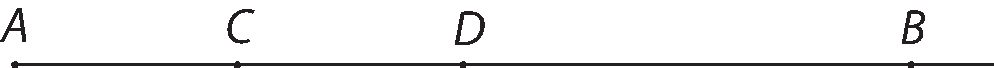
\includegraphics[trim = 0mm -3mm 0mm 0mm, clip, width=0.55\textwidth]{images/LH035,14,02_112r-d1.pdf}\\
\noindent \centering [\textit{Fig. 6}]\edtext{}{\lemma{\hspace{1.3mm}[\textit{Fig. 6}]}\killnumber\Cfootnote{\cite{00311}Siehe a.a.O., Tafel der Abbildungen, Fig. 10.}}%
\pend
\vspace{1.5em} 
\pstart
\edtext{\textso{Prop. 18. }%
Si  \setline{12}deux boules\protect\index{Sachverzeichnis}{boule} dont l'une est triple de l'autre
\textit{se choquent \edtext{avec des}{\lemma{avec}\Bfootnote{%
\textit{(1)}\ une
\textit{(2)}\ \textit{des}
\textit{L}}}
vistesses egales et uniformes,}
la plus grande \textit{après le choc\protect\index{Sachverzeichnis}{choc} demeurera
en repos et la moindre $\displaystyle B$ retournera en arriere avec une vitesse double de celle qu'elle avoit
avant le choc.\protect\index{Sachverzeichnis}{choc}}%
}{\lemma{12-15 \hspace{1.8mm}\textso{Prop. 18}. [...] \textit{choc}}\killnumber\Cfootnote{\cite{00311}a.a.O., S. 112. Zitat mit Auslassungen.}}
\pend
\pstart
\edtext{\textit{Il s'ensuit que si deux corps à ressort,\protect\index{Sachverzeichnis}{ressort}
inegaux se choquent directement avec des vitesses egales\protect\index{Sachverzeichnis}{vitesse}
et que le poids\protect\index{Sachverzeichnis}{poids} du plus pesant soit plus que triple du poids de l'autre,
ils s'avanceront tous deux après le choc\protect\index{Sachverzeichnis}{choc} selon la direction du plus pesant,
et que s'il est moins que triple}[,]
\textit{chacun de ces corps retournera en arrière.}%
}{\lemma{\textit{Il s'ensuit} [...] \textit{en arrière}}\Cfootnote{\cite{00311}a.a.O., S. 114.\hspace{15mm}}}
\pend
\pstart
\edtext{\textso{Prop. 19. }%
\textit{Si une ligne comme}
[$\displaystyle AB$]\edtext{}{\lemma{$\displaystyle AC$}\Bfootnote{\textit{L ändert Hrsg. nach Vorlage}}}
\textit{est divisée au point $\displaystyle C$
en la raison reciproque des poids des corps $\displaystyle A$ et $\displaystyle B,$
et aussi au point $\displaystyle D$ selon la raison des vistesses\protect\index{Sachverzeichnis}{vitesse}
avec lesquelles ils se chocquent,
c'est à dire que si $\displaystyle BC$ est à $\displaystyle CA$
comme le poids\protect\index{Sachverzeichnis}{poids} du corps $\displaystyle A$ est au poids du corps $\displaystyle B,$
et que $\displaystyle AD$ soit à $\displaystyle BD$
comme la vistesse du corps $\displaystyle A,$ à la vistesse du corps $\displaystyle B,$
et que $\displaystyle CE$ soit faite egale à $\displaystyle CD,$
la ligne $\displaystyle EA$ sera la vitesse du corps $\displaystyle A$
selon la direction de $\displaystyle E$ vers $\displaystyle A,$
et $\displaystyle EB$ la vitesse du corps $\displaystyle B$
selon la direction de $\displaystyle E$ vers $\displaystyle B$ après leur chocq\protect\index{Sachverzeichnis}{choc}}
par la prop. 13. et 2\textsuperscript{de} consequence de la prop. 15.}{\lemma{\textso{Prop. 19}. [...] prop. 15}\Cfootnote{\cite{00311}a.a.O., S. 115f.}}
\pend
\pstart
\noindent
\centering
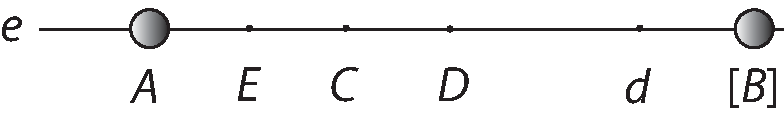
\includegraphics[trim = 0mm -3mm 0mm 0mm, clip, width=0.45\textwidth]{images/LH035,14,02_112r-d2.pdf}\\
\noindent \centering [\textit{Fig. 7}]\edtext{}{\lemma{\hspace{1.8mm}[\textit{Fig.~7}]}\killnumber\Cfootnote{\cite{00311}Fehlende Bezeichnung nach Vorlage ergänzt. Siehe a.a.O., Tafel der Abbildungen, Fig. 13.}}%
\pend
\vspace{1.5em}
\pstart
\edtext{\textso{Prop. 20. }%
Si \setline{1}deux corps à
[ressort]\protect\index{Sachverzeichnis}{ressort}\edtext{}{\lemma{ressorts}\Bfootnote{\textit{L ändert Hrsg.}}}
se sont choqués directement,
\textit{et qu'ils se choquent une seconde fois,
avec les vistesses acquises par le premier chocq,
ils reprendront après le second chocq la même vitesse propre ou le repos,
que chacun avoit avant le premier}
\edtext{\textit{chocq\protect\index{Sachverzeichnis}{choc}.}
N'importe}{\lemma{\textit{chocq.}}\Bfootnote{%
\textit{(1)}\ La même
\textit{(2)}\ N'importe
\textit{L}}}
si les corps sont egaux ou inegaux,
item si tous deux sont en mouuement,
\edtext{ou si l'un}{\lemma{ou si}\Bfootnote{%
\textit{(1)}\ quelques uns
\textit{(2)}\ l'un
\textit{L}}}
est en repos.%
}{\lemma{\hspace{1.8mm}1-5 \hspace{1.8mm}\textso{Prop. 20}. [...] repos}\killnumber\Cfootnote{\cite{00311}a.a.O., S. 122.}}
\pend
\pstart
\edtext{\textso{Prop. 21. }%
\textit{Si deux corps à ressort (egaux ou inegaux) se choquent directement avec des vitesses (egales ou inegales) ils se separeront
après le chocq\protect\index{Sachverzeichnis}{choc} avec la même vitesse respective,
avec laquelle ils se sont rencontrez.}
Par ce que la vitesse respective\protect\index{Sachverzeichnis}{vitesse respective}
\textit{produite par la force des ressorts\protect\index{Sachverzeichnis}{force de ressort}
est tousjours la même}
avec \textit{celle}
\edtext{\textit{qui a produit}
\edtext{le ressort.}{\lemma{le ressort}\Cfootnote{In der Vorlage \textit{les ressorts}.}}%
}{\lemma{\textit{qui}}\Bfootnote{%
\textit{(1)}\ est produite par \textit{les ressorts}
\textit{(2)}\ \textit{a produit} le ressort.
\textit{L}}}%
}{\lemma{\textso{Prop. 21}. [...] ressort}\Cfootnote{\cite{00311}a.a.O., S.~126f.}}
\pend
\pstart
\edtext{\textso{Prop. 22. }%
\textit{Si un corps à ressort\protect\index{Sachverzeichnis}{ressort}
chocque directement un autre corps à ressort,
soit que le corps chocqué soit en repos,
soit qu'il s'avance de
même part que l'autre selon une même ligne de direction,
la somme des quantitez de mouuement\protect\index{Sachverzeichnis}{quantité de mouvement} de deux ensemble
après le choc\protect\index{Sachverzeichnis}{choc} sera la même, qu'avant le chocq,
s'ils s'avancent tous deux ou si celuy qui a chocqué demeure sans mouuement;
mais si ce dernier corps retourne en arriere,
la quantité de mouuement\protect\index{Sachverzeichnis}{quantité de mouvement} de celuy qui s'avance sera plus grande,
que celle qu'avoit le corps, qui s'est meu seul,
ou les deux meus de même part avant le chocq;\protect\index{Sachverzeichnis}{choc}
et l'excès sera egal à la quantité de mouuement de celuy qui retourne en arriere.}%
}{\lemma{\textso{Prop. 22}. [...] \textit{en arriere}}\Cfootnote{\cite{00311}a.a.O., S. 128f.}}
\pend
\pstart
\edtext{\textso{Prop. 23. }%
\textit{Si deux corps inegaux à ressort se chocqent directement
avec des vistesses contraires non reciproques à leurs poids,\protect\index{Sachverzeichnis}{poids}
et qu'ils s'avancent tous deux,
ou que l'un d'eux demeure en repos après le chocq,
la somme de}
[\textit{leurs}]\edtext{}{\lemma{leur}\Bfootnote{\textit{L ändert Hrsg. nach Vorlage}}}
\textit{quantités de mouuement\protect\index{Sachverzeichnis}{quantité de mouvement} après le chocq,\protect\index{Sachverzeichnis}{choc}
sera égale à la difference de}
[\textit{celles}]\edtext{}{\lemma{celle}\Bfootnote{\textit{L ändert Hrsg. nach Vorlage}}}
\textit{qu'ils avoient avant le chocq.
Mais si les deux corps retournent en arriere après
\edtext{s'estre chocquez,}{\lemma{s'estre}\Bfootnote{%
\textit{(1)}\ \textit{chocqués}
\textit{(2)}\ \textit{chocquez,}
\textit{L}}}
la somme de}
[\textit{leurs}]\edtext{}{\lemma{leur}\Bfootnote{\textit{L ändert Hrsg. nach Vorlage}}}
\textit{quantités de mouuement sera plus grande que cette difference,
et l'excès sera egal au double de la quantité}
[\textit{de mouvement}]\edtext{}{\lemma{\textit{de mouvement}}\Bfootnote{\ \textit{erg. Hrsg. nach Vorlage}}}
\textit{de celuy à qui il en reste le moins.}%
}{\lemma{\textso{Prop. 23}. [...] \textit{le moins}}\Cfootnote{\cite{00311}a.a.O., S. 131f.}}
\pend
%
\pstart
\edtext{\textso{Prop. 24. }%
\textit{Si le poids\protect\index{Sachverzeichnis}{poids} d'un corps à ressort\protect\index{Sachverzeichnis}{ressort} est triple,
ou moins que triple du poids d'un autre corps à ressort moindre,
et qu'ils se chocquent avec des vitesses egales,\protect\index{Sachverzeichnis}{vitesse}
la somme de leurs quantités de mouuement\protect\index{Sachverzeichnis}{quantité de mouvement}
après le chocq sera moindre qu'avant le chocq,\protect\index{Sachverzeichnis}{choc}
\edtext{et la difference sera}{\lemma{}\Bfootnote{\textit{et la difference}\ \textbar\ du corps\ \textit{gestr.}\ \textbar\ \textit{sera\ L}}}
egale au quarré de la difference du poids de deux corps
si leur vitesse respective\protect\index{Sachverzeichnis}{vitesse respective} est exprimée par la somme
de \edtext{leurs poids}{\lemma{\textit{leurs}}\Bfootnote{\textbar\ propres\ \textit{gestr.}\ \textbar\ \textit{poids\ L}}}.}%
}{\lemma{\textso{Prop. 24}. [...] \textit{poids}}\Cfootnote{\cite{00311}a.a.O., S. 137.}}
\pend
%
\pstart
\edtext{\textso{Prop. 25. }%
\textit{S'il y a deux corps inegaux à ressort,
$\displaystyle A$ et $\displaystyle B$,
et que le moindre $\displaystyle B$
estant en repos, soit choqué directement par le plus pesant,
avec une vitesse, dont les degrez}
[\textit{soient}]\edtext{}{\lemma{soit}\Bfootnote{\ \textit{L ändert Hrsg. nach Vorlage}}}
\textit{exprimés par le nombre
qui exprime la somme des poids des deux corps,
le corps $\displaystyle B$ après le chocq\protect\index{Sachverzeichnis}{choc}
aura une vitesse\protect\index{Sachverzeichnis}{vitesse}
dont les degrez seront exprimés par un nombre
double du nombre du plus grand poids,\protect\index{Sachverzeichnis}{poids}
et les degrez de vitesse que le corps $\displaystyle A$ perdra
seront exprimés par le double du nombre du moindre poids.}%
}{\lemma{\textso{Prop. 25}. [...] \textit{poids}}\Cfootnote{\cite{00311}a.a.O., S. 142f.\hspace{15mm}}}
%
[112~v\textsuperscript{o}]%%%%%%%%%% HIER BEGINNT BLATT 112v.
%
\pend
\pstart
\edtext{\textso{Prop. 26. }\protect\label{LH035,14,02_112v-ref1}%
\textit{S'il y a deux corps inegaux à ressort $\displaystyle A$ et $\displaystyle B$,
et que le plus pesant $\displaystyle A$ estant en repos
soit chocqué par le plus leger avec une vitesse\protect\index{Sachverzeichnis}{vitesse}
dont les degrez soient exprimés par le nombre
qui exprime la somme des poids des deux corps:
le corps $\displaystyle A$ après le chocq aura une quantité de mouuement\protect\index{Sachverzeichnis}{quantité de mouvement}
double de celle du corps $\displaystyle B$ avant le chocq\protect\index{Sachverzeichnis}{choc}
\edtext{diminuée du quarré du nombre,}{\lemma{diminuée du}\Bfootnote{%
\textit{(1)}\ \textit{nombre}
\textit{(2)}\ \textit{quarré du nombre,}
\textit{L}}}
qui exprime le poids\protect\index{Sachverzeichnis}{poids}
du corps $\displaystyle B,$
et les degrez de vitesse que le corps $\displaystyle B$ perdra
seront exprimés par le double du nombre
qui exprime son poids.}%
}{\lemma{\textso{Prop. 26}. [...] \textit{poids}}\Cfootnote{\cite{00311}a.a.O., S. 146.}}
\pend
\pstart
\edtext{On voit par là,
et par \textit{la precedente, et il est aisé de
\edtext{le}{\lemma{le}\Bfootnote{\textit{erg. L}}}
demonstrer universellement
que lorsque les poids demeurent les mêmes
quelque soit le corps qui chocque}[,]
\textit{sa vitesse restante est tousjours la même,
et la quantité de mouuement\protect\index{Sachverzeichnis}{quantité de mouvement}
du corps chocqué est aussi la même.
La seule difference est que la vitesse\protect\index{Sachverzeichnis}{vitesse}
qui reste au plus grand corps est en avant,
et celle} qui reste au
\edtext{\textit{moindre en arriere.}}{\lemma{}\Bfootnote{%
\textit{moindre}\ \textbar\ est \textit{gestr.}\ \textbar\ \textit{en arriere.}\ \textit{L}}}%
}{\lemma{On voit [...] \textit{en arriere}}\Cfootnote{\cite{00311}a.a.O., S. 150f. Zitat mit Auslassung.}}
\pend
\pstart
\edtext{\textso{Premiere consequence: }%
\textit{Il suit des deux propositions precedentes
que le corps chocqué prend autant de vitesse
et de quantité de mouuement\protect\index{Sachverzeichnis}{quantité de mouvement}
par le mouuement simple,
que par le mouuement de ressort.\protect\index{Sachverzeichnis}{ressort}}%
}{\lemma{\textso{Premiere} [...] \textit{ressort}}\Cfootnote{\cite{00311}a.a.O., S. 151.\hspace{35mm}}}
\pend
\pstart
\edtext{\textso{2\textsuperscript{\textso{\,de}}\! consequence, }%
\textit{il s'ensuit aussi,
que si l'on prend deux corps inegaux à ressort
de tel poids\protect\index{Sachverzeichnis}{poids} qu'on voudra,
et que l'un des deux estant en repos,
soit chocqué par l'autre directement,
avec une vitesse egale au nombre de la somme de leurs poids,
la somme de leurs vitesses après le chocq,\protect\index{Sachverzeichnis}{choc}
sera triple de cette premiere vitesse,\protect\index{Sachverzeichnis}{vitesse}
moins quatre fois le nombre du moindre poids,
si c'est le moindre corps qui soit en repos;
et si c'est le plus \edtext{grand,
la somme de leurs quantitez de mouuement après le chocque sera}{\lemma{grand,}\Bfootnote{%
\textit{(1)}\ \textit{ce sera}
\textit{(2)}\ \textit{la somme} [...] \textit{sera}
\textit{L}}}
triple de la quantité de mouuement\protect\index{Sachverzeichnis}{quantité de mouvement}
du moindre corps avant le chocq,\protect\index{Sachverzeichnis}{choc}
moins 4 fois le quarré du nombre du moindre poids.}%
}{\lemma{\textso{2}\textsuperscript{\textso{\,de}} \textso{consequence} [...] \textit{poids}}\Cfootnote{\cite{00311}a.a.O., S. 151f.}}
\pend
\count\Afootins=1400
\count\Bfootins=1400
\count\Cfootins=1400
\pstart
\edtext{\textit{Supposons que le corps $\displaystyle A$ pese 100,000 onces,
et le corps $\displaystyle B$ une once,
or si c'est le moindre corps qui chocque}[,]
\textit{sa vitesse premiere sera 100,001
et la quantité de mouuement du corps chocqué sera 200,000
et celle qui restera dans le moindre corps sera 99999,
dont la somme sera triple de la premiere quantité de mouuement du moindre corps,
à s\c{c}avoir % ?????
\edtext{10,000}{\lemma{10,000}\Cfootnote{So auch in der Vorlage. Eigentlich sollte es \textit{100,001} heißen.}}\edtext{,}{\lemma{}\Afootnote{\textit{Über 10,000:} \Denarius}}
moins 4,
c'est à dire quatre fois le quarré de l'unité
qui marque le moindre poids.\protect\index{Sachverzeichnis}{poids}
Mais si le moindre corps est en repos}[,]
\textit{sa vitesse\protect\index{Sachverzeichnis}{vitesse}
après le chocq\protect\index{Sachverzeichnis}{choc} sera 200,000,
et celle de l'autre, 99999, dont la somme est aussi 3ple moins 4 de 100001.%
\edtext{}{\lemma{}\Afootnote{\textit{Am Rand:} NB.\vspace{-4mm}}}%
\\%
\hspace*{7,5mm}%
On voit par cet
\edtext{exemple qu'on}{\lemma{exemple}\Bfootnote{%
\textit{(1)}\ que l
\textit{(2)}\ \textit{qu'on}
\textit{L}}}
peut tellement augmenter l'inegalité des poids de ces corps,
que la somme de leurs quantitez de mouuement\protect\index{Sachverzeichnis}{quantité de mouvement}
ou de leurs vitesses après le chocq sera triple de la premiere,
moins une de ses parties plus}
[\textit{petite}]\edtext{}{\lemma{petites}\Bfootnote{\ \textit{L ändert Hrsg. nach Vorlage}}}
\textit{qu'aucune qu'on puisse dire.%
\\%
\hspace*{7,5mm}%
Cette seconde consequence doit passer pour un \textso{paradoxe} assez surprenant.
Car comment un corps peut il donner une plus grande vitesse\protect\index{Sachverzeichnis}{vitesse}
ou une plus grande quantité de mouuement
à un autre corps, que celle qu'il a,
et conserver la sienne presque tout}[']\textit{enti\-ere?
Mais cette merveille procede de deux regles de la nature
expliquées dans} la proposition 5\textsuperscript{\,me} et dans la prop. troisieme[,]
\textit{s\c{c}avoir que l'impression mutuelle de deux corps l'un sur l'autre est tousjours la même,
quand la vitesse respective\protect\index{Sachverzeichnis}{vitesse respective}
avec laquelle ils se rencontrent directement est la même,
et quand ils se font mis en ressort,\protect\index{Sachverzeichnis}{ressort}
par leur chocq,\protect\index{Sachverzeichnis}{choc}
ils partagent leur vitesse respective en raison reciproque de leurs poids,
ce qui fait que quand c'est le plus grand corps qui chocque}[,]
\textit{les vitesses sont augmentées
et les quantitez de mouuement demeurent egales;
et quand c'est le moindre corps}[,]
\textit{les quantitez de mouuement\protect\index{Sachverzeichnis}{quantité de mouvement}
sont augmentées et la somme des vitesses demeure égale.
%
\count\Afootins=1000
\count\Bfootins=1000
\count\Cfootins=1000
\\%
\hspace*{7,5mm}%
Pour faire voir par l'experience qu'un petit corps
chocqué par un plus grand re\c{c}oit presque le double de sa vitesse,\protect\index{Sachverzeichnis}{vitesse}
il faut \edtext{suspendre deux}{\lemma{}\Bfootnote{\textit{suspendre}\ \textbar\ presque \textit{streicht Hrsg.}\ \textbar\ \textit{deux\ L}}}
boules d'ivoire\protect\index{Sachverzeichnis}{ivoire} fort inegales en poids,\protect\index{Sachverzeichnis}{poids}
comme} \edtext{par exemple}{\lemma{par exemple}\Bfootnote{\textit{erg. L}}}\edtext{}{\lemma{par exemple}\Cfootnote{Siehe die Abbildung [\textit{Fig. 8}].}}
\textit{si} [\textit{l'une}]\edtext{}{\lemma{l'un}\Bfootnote{\textit{L ändert Hrsg. nach Vorlage}}}
\textit{pese 4 gros, il faut que l'autre en pese 80;
elevez la plus grosse $\displaystyle G$ jusqu'à 84
\edtext{degrez, afin}{\lemma{}\Bfootnote{\textit{degrez,}\ \textbar\ \textit{adjoutant 54 degrez à l'arc $\displaystyle LM$,}\ \textit{gestr.}\ \textbar\ \textit{afin\ L}}}
d'avoir une vitesse respective\protect\index{Sachverzeichnis}{vitesse respective}
egale au nombre qui exprime la somme des poids,
laissez aller cette boule contre l'autre\protect\index{Sachverzeichnis}{boule}
en sorte qu'elle la chocque directement,
et vous verrez que la petite boule ira de telle force,\protect\index{Sachverzeichnis}{force}
qu'elle fera deux ou trois tours à l'entour des deux clouds
si elle ne rencontre rien.
Or par ce \edtext{qui a esté}{\lemma{qui}\Bfootnote{%
\textit{(1)}\ est
\textit{(2)}\ \textit{a esté}
\textit{L}}}
dit, elle doit receuuoir une vitesse double de celle
qui la feroit remonter par un arc de cercle de}
\edtext{84}{\lemma{84}\Cfootnote{In der Vorlage \textit{quatre vingts}.\hspace{15mm}}}
\textit{degrez, ou qui la feroit elever perpendiculairement à
\edtext{environ 40}{\lemma{environ}\Bfootnote{%
\textit{(1)}\ 80
\textit{(2)}\ \textit{40}
\textit{L}}}
pouces de hauteur,
si les filets de suspension sont de 4 pieds,
et par consequent elle remonteroit à environ 13 pieds
de bas en haut par cette vitesse double,
par la 2\textsuperscript{\,de} supposition;
donc elle remonteroit plus haut,
que le diametre entier du cercle du pendule;
mais estant retenue par le filet,
qui l'empeche de monter plus haut que 8 pieds,
elle employera en rond le reste de sa vitesse,\protect\index{Sachverzeichnis}{vitesse}
qui luy fera faire deux ou 3 tours à l'entour des}
deux \textit{clouds,
nonobstant la resistence de l'air.}%
}{\lemma{\textit{Supposons} [...] \textit{de l'air}}\Cfootnote{\cite{00311}a.a.O., S. 152-157. Zitat mit Auslassungen.}}
\pend
%%
%\pstart
%\vspace{2em}% PR: Rein provisorisch !!!
%\noindent
%\centering
%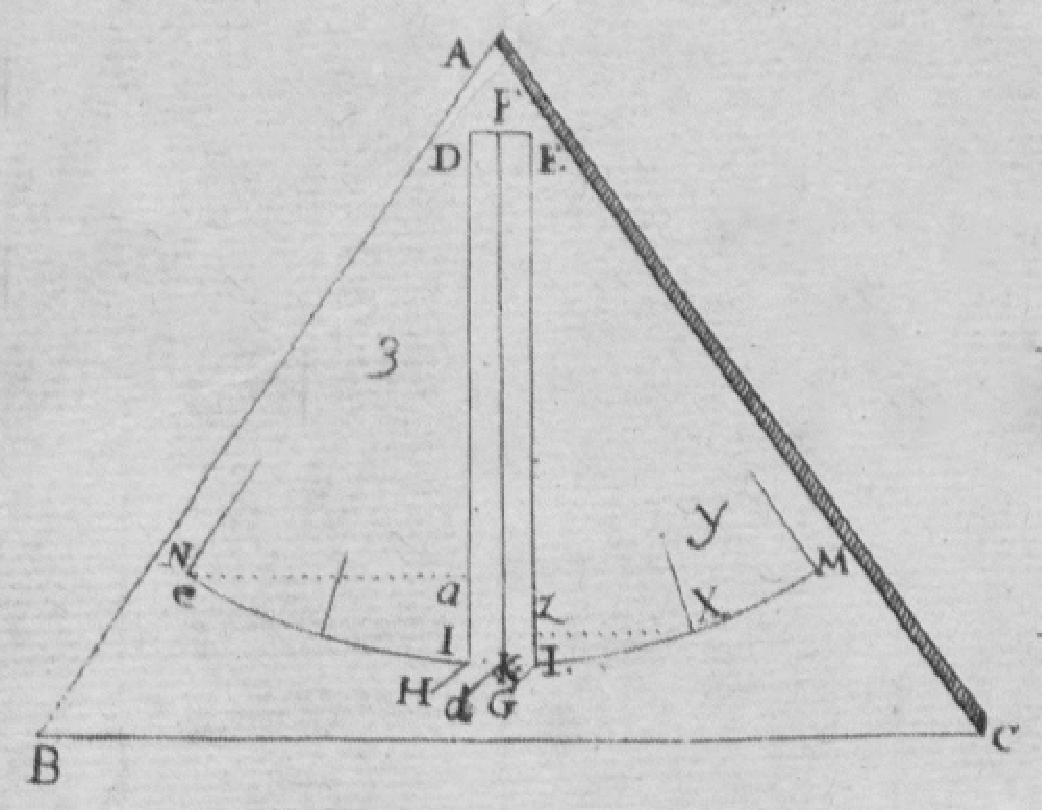
\includegraphics[trim = 0mm -3mm 0mm 0mm, clip, width=0.632\textwidth]{images/Mariotte_1673_Fig-3.pdf}\\
%\noindent \centering [\textit{Fig. 8; erg. Hrsg. nach Mariotte}]\label{LH035,14,02_112v-ref2}%
%\edtext{}{\lemma{\ [\textit{Fig. 8}]}\killnumber\Cfootnote{\cite{00311}Siehe a.a.O., Tafel der Abbildungen, Fig. 3.}}
%\pend
%\newpage
%\vspace{1.5em}% PR: Rein provisorisch !!!
\count\Afootins=1000
\count\Bfootins=1000
\count\Cfootins=1000
%%%%%%%%%%%%%%%%%%%% 
\pstart
\edtext{\textso{3\textsuperscript{\textso{\,me}}\! consequence. }
\textit{Il suit aussi de ces deux propositions,
que si deux corps à ressort\protect\index{Sachverzeichnis}{ressort}
sont fort inegaux en poids,\protect\index{Sachverzeichnis}{poids}
ils peuuent se rencontrer directement de telle sorte
que leurs secondes quantitez de mouuement\protect\index{Sachverzeichnis}{quantité de mouvement}
ou leurs secondes vitesses ne seront à fort peu près,
que le tiers des premieres.
C'est à  dire qu'il se perdra à fort peu près les deux tiers de leurs vitesses\protect\index{Sachverzeichnis}{vitesse}
ou de leurs quantitez de mouuement par le chocq.\protect\index{Sachverzeichnis}{choc}
Car si les deux corps $\displaystyle A$ et $\displaystyle B$
\edtext{cy dessus}{\lemma{cy dessus}\Cfootnote{Siehe oben, S.~\pageref{LH035,14,02_112v-ref1}.}}
se chocquent une seconde fois avec les vitesses acquises par le premier chocq,
il n'en restera qu'un seul en mouuement après le}
[\textit{seconde}]\edtext{}{\lemma{\textit{seconde}}\Bfootnote{\ \textit{erg. Hrsg. nach Vorlage}}}
\textit{chocq par la 20\textsuperscript{\,me} prop.
et il reprendra la même vitesse et la même quantité de mouuement
qu'il avoit avant le premier chocq.\protect\index{Sachverzeichnis}{choc}
Donc comme le premier chocq} l'a fait tripler,
de même le second deminuera des 2 tiers la quantité de mouuement.\protect\index{Sachverzeichnis}{quantité de mouvement}}%
{\lemma{\textso{3}\textsuperscript{\textso{\,me}} [...] mouuement}\Cfootnote{\cite{00311}a.a.O., S. 157f. Zitat mit Auslassungen.}}
\pend
\pstart
%\vspace{2em}% PR: Rein provisorisch !!!
\noindent
\centering
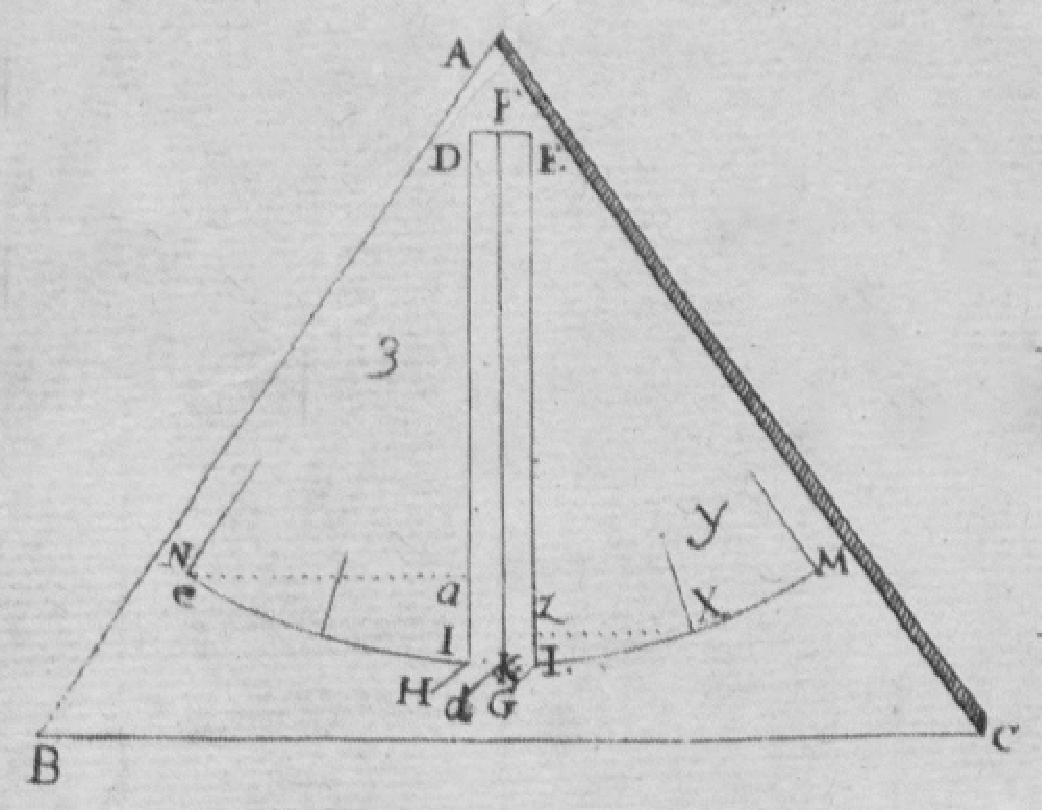
\includegraphics[trim = 0mm -3mm 0mm 0mm, clip, width=0.632\textwidth]{images/Mariotte_1673_Fig-3.pdf}\\
\noindent \centering [\textit{Fig. 8; erg. Hrsg. nach Mariotte}]\label{LH035,14,02_112v-ref2}%
\edtext{}{\lemma{\ [\textit{Fig. 8}]}\killnumber\Cfootnote{\cite{00311}Siehe a.a.O., Tafel der Abbildungen, Fig. 3.}}
\pend
\vspace{1.5em}
\pstart
% PR: Rein provisorisch!
\centering % PR: Bitte, korrekt setzten. Danke.
[\textit{Teil 2}]
\pend
\vspace{0.5em}
\pstart
\noindent%
Quaecunque \setline{2}hactenus dicta sunt,
demonstrari fere possunt ex principiis duobus,
quorum unum est:
Vires\protect\index{Sachverzeichnis}{vis corporis}
\edtext{corporum}{\lemma{corporum}\Bfootnote{\textit{erg. L}}}
esse in composita
\edtext{ratione celeritatum\protect\index{Sachverzeichnis}{celeritas}
et magnitudinum,\protect\index{Sachverzeichnis}{magnitudo}}{\lemma{ratione}\Bfootnote{%
\textit{(1)}\ magnitudinum co
\textit{(2)}\ ex celeritatibus et magnitudinibus corporum agentium
\textit{(3)}\ ex rationibus celeritatum et magnitudinum
\textit{(4)}\ celeritatum et magnitudinum,
\textit{L}}}
alterum[:] corpora reflectentia
\edtext{eadem vi sejungi qua concurrere.}{\lemma{eadem}\Bfootnote{%
\textit{(1)}\ celeritate sejungi qua
\textit{(a)}\ convenere
\textit{(b)}\ concurrere
\textit{(2)}\ vi sejungi qua concurrere.
\textit{L}}}
Quae duo principia
\edtext{velut experimentis\protect\index{Sachverzeichnis}{experimentum} explorata}{\lemma{velut}\Bfootnote{%
\textit{(1)}\ phenomena\protect\index{Sachverzeichnis}{phaenomenon}
\textit{(2)}\ experimentis explorata
\textit{L}}}
sumi possunt, etsi habeant demonstrationes
\edtext{suas; primum ex natura systematis,
2\textsuperscript{dum} ex Elaterii\protect\index{Sachverzeichnis}{elaterium} natura.}{\lemma{suas;}\Bfootnote{%
\textit{(1)}\ alterum ex natura Elaterii, pr
\textit{(2)}\ primum [...] Elaterii natura.
\textit{L}}}
\pend
\pstart
Caeterum quae verbis lineisve expressa sunt
\edtext{ea longe simplicius promtiusque ad usum}{\lemma{ea}\Bfootnote{%
\textit{(1)}\ facilius
\textit{(2)}\ longe [...] usum
\textit{L}}}
symbolis exhibentur.
Hoc enim facto nullo negotio definiuntur,
quae alioquin vix ambagibus multis demonstrari possunt.
\pend
\pstart
Itaque quoniam non nisi cum duobus corporibus nobis negotium est,
appellemus, unum $\displaystyle a,$
alterum $\displaystyle e.$
Celeritatem corporis $\displaystyle a,$ appellemus $\displaystyle b,$
et celeritatem corporis $\displaystyle e,$ appellemus $\displaystyle c.$
Vis corporis $\displaystyle a$ erit $\displaystyle \sqcap\ ab,$
et vis corporis $\displaystyle e,$ erit $\displaystyle ec.$
Celeritas respectiva corporum, qua ad se invicem accedunt,
vel a se invicem \edtext{recedunt,
quodammodo fiet ex absolutis. Pone enim}{\lemma{recedunt,}\Bfootnote{%
\textit{(1)}\ erit, summa vel differentia absolutarum, nempe $\displaystyle \pPsMs ab\ \pPsMsPs ec.$
%%%%%%%%%%%%%%%%%%%%%%%%%%%%%%%%%%%%%%
\protect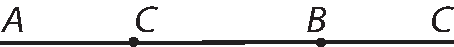
\includegraphics[width=0.27\textwidth]{images/LH035,14,02_112v-d2.pdf}%
%%%%%%%%%%%%%%%%%%%%%%%%%%%%%%%%%%%%%%
\ \textit{(a)}\ Erit celeritas respectiva $\displaystyle AB$
\textit{(b)}\ Pone enim celeritates absolutas esse $\displaystyle AC,$ $\displaystyle BC,$ erit
\textit{(2)}\ quodammodo fiet ex 
\textit{(a)}\ respectivis
\textit{(b)}\ absolutis. Pone enim
\textit{L}}}
corpora sibi occurrere, $\displaystyle A$ et $\displaystyle B,$ in puncto $\displaystyle C.$
%%%%%%%%%%%%%%%%%%%%%%%%%%%%%%%%%%%%%%
\protect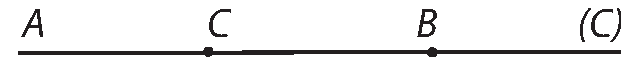
\includegraphics[width=0.42\textwidth]{images/LH035,14,02_112v-d3.pdf}\\%
\vspace{-1em}
%%%%%%%%%%%%%%%%%%%%%%%%%%%%%%%%%%%%%%
\pend
\count\Afootins=1200
\count\Bfootins=1200
\count\Cfootins=1200
%\newpage
\pstart
\noindent
Utique \setline{3}manifestum est si fingamus hominem insistere corpori $\displaystyle A,$
ei corpus $\displaystyle A$ immobile appariturum,
et $\displaystyle B$ solum accedere ad ipsum celeritate quae sit ut $\displaystyle AB$[,]
sin ponamus corpus $\displaystyle B$ praecedere et corpus $\displaystyle A$ insequi,
et punctum assecutionis esse in $\displaystyle (C).$
Fingamus iterum hominem esse in corpore $\displaystyle B,$
qui oculos in nil nisi in corpus $\displaystyle A$
[defixos]\edtext{}{\lemma{defixum}\Bfootnote{\textit{L ändert Hrsg.}}}
habeat, aut in plano per omnia simili,
\edtext{velut glacie perfecte polita, quousque}{\lemma{velut}\Bfootnote{%
\textit{(1)}\ aqua
\textit{(2)}\ glacie perfecte polita\ \textbar\ polita \textit{streicht Hrsg.}\ \textbar\ , quousque
\textit{L}}}
oculi acies extenditur diffusa, constitutum esse,
perinde utique ipsi erit,
ac si $\displaystyle B$ fuisset initio in $\displaystyle C,$
ac proinde celeritas respectiva erit eo casu [$\displaystyle AC$].\edtext{}{\lemma{$\displaystyle A(C)$}\Bfootnote{\textit{L ändert Hrsg.}}}
\pend
\pstart
Sed jam video hoc non procedere,
ita enim etiam priore casu
\edtext{linea $\displaystyle AC$ repraesentabit}{\lemma{linea $\displaystyle AC$}\Bfootnote{%
\textit{(1)}\ erit
\textit{(2)}\ repraesentabit
\textit{L}}}
vim respectivam, et alia atque alia ejus quantitas erit,
prout hanc vel illam ut immobilem
\edtext{eliges. Nam si}{\lemma{eliges.}\Bfootnote{%
\textit{(1)}\ Si
\textit{(2)}\ Nam si
\textit{L}}}
in \edtext{corpore $\displaystyle A(B)$}{\lemma{corpore}\Bfootnote{%$
\textit{(1)}\ $\displaystyle A$
\textit{(2)}\ $\displaystyle ADE$
\textit{(3)}\ $\displaystyle ATE$
\textit{(4)}\ $\displaystyle A(B)$
\textit{L}}}
constitutum ponas et
\edtext{corpus
%
[113~r\textsuperscript{o}] %%%%%%%%%% HIER BEGINNT BLATT 113r.
%
$\displaystyle A(B)$}{\lemma{corpus}\Bfootnote{%
\textit{(1)}\  $\displaystyle A$
\textit{(2)}\ $A(B)$
\textit{L}}}
proinde immobile fingas,
statimque constitutum in $\displaystyle C,$
\edtext{utique tempore}{\lemma{}\Bfootnote{%
utique\ \textbar\ utique \textit{streicht Hrsg.}\ \textbar\ tempore \textit{L}}}
\edtext{accessionis a corpore $\displaystyle B(A)$}{\lemma{accessionis a}\Bfootnote{%
\textit{(1)}\ recta $\displaystyle B$
\textit{(2)}\ corpore
\textit{(a)}\ $\displaystyle B$
\textit{(b)}\ $\displaystyle B(A)$
\textit{L}}}
percurri apparebit \edtext{spatium\protect\index{Sachverzeichnis}{spatium} $\displaystyle BC.$
Verum si aliter fiat fictio, nimirum, corpus $\displaystyle B$%
}{\lemma{spatium $\displaystyle BC.$}\Bfootnote{%
\textit{(1)}\ Contra si $\displaystyle B$ pon
\textit{(2)}\ Verum [...] corpus $\displaystyle B$ 
\textit{L}}}
\edtext{immobile esse%
}{\lemma{immobile}\Bfootnote{%
\textit{(1)}\ manere $\displaystyle (AC)$
\textit{(2)}\ \textbar\ $\displaystyle (AC)$ \textit{streicht Hrsg.}\ \textbar\ esse
\textit{L}}}
in loco $\displaystyle B,$
perinde ac si totus reliquus mundus ad ipsum referendus esset,
tunc tempore accessionis a corpore $\displaystyle A$ percurretur spatium $\displaystyle AB,$
celeritate\protect\index{Sachverzeichnis}{celeritas}
\edtext{scilicet, quae sit ad propriam ejus
ut $\displaystyle AB$ est ad $\displaystyle AC.$}{\lemma{scilicet,}\Bfootnote{%
\textit{(1)}\ quanta est $\displaystyle AC$
\textit{(2)}\ quae [...] ad $\displaystyle AC.$
\textit{L}}}
Eodem modo de $\displaystyle BC.$
Idemque est si intelligas punctum adhiberi $\displaystyle (C)$
extra lineam $\displaystyle AB,$ pro puncto $\displaystyle C.$
Maneat \edtext{ergo celeritatem%
}{\lemma{ergo}\Bfootnote{%
\textit{(1)}\ vim
\textit{(2)}\ celeritatem
\textit{L}}}
respectivam exprimi ad absolutas, ratione distantiae corporum $\displaystyle AB,$
ad \edtext{ipsas $\displaystyle AC,$ vel $\displaystyle BC,$%
}{\lemma{ipsas}\Bfootnote{%
\textit{(1)}\ $\displaystyle AB,$ vel
\textit{(2)}\ $\displaystyle AC,$ vel $\displaystyle BC,$
\textit{L}}}
vel $\displaystyle A(C)$ vel $\displaystyle B(C).$
Quod si ergo celeritatem respectivam\protect\index{Sachverzeichnis}{celeritas respectiva}
appellemus $\displaystyle r,$
erit $\displaystyle r\, \sqcap\, +\, b\, + c,$
vel $\displaystyle r\, \sqcap\, +\, b\, - c,$
vel $\displaystyle r\, \sqcap\, -\, b\, + c,$
sive $\displaystyle \underline{r}\, \sqcap\, (\alpha\alpha\omega)b\, (\alpha\omega\alpha)c$
eritque $\displaystyle \underline{b}\, \sqcap\, (\alpha\alpha\omega)r\, (\omega\alpha\alpha)c,$
et $\displaystyle \underline{c}\, \sqcap\, (\alpha\omega\alpha)r\, (\omega\alpha\alpha)b.$
Quod si placet characteribus ita exprimi potest:\
$\displaystyle \underline{r}\ \sqcap\ \pPsPsMs b\ \pPsMsPs c,\ $
$\displaystyle \underline{b}\ \sqcap \!\efrac{\vphantom{+}}{\displaystyle \efrac{\displaystyle +}{\efrac{\displaystyle +}{\displaystyle -}}}r \efrac{\vphantom{+}}{\displaystyle \efrac{\displaystyle -}{\efrac{\displaystyle +}{\displaystyle +}}}c,$\
vel $\displaystyle \pPsPsMs r\ \pMsPsPs c,$
vel quia
$\displaystyle r\, \sqcap\!\! \efrac{\vphantom{+}}{\efrac{\displaystyle +}{\efrac{\scriptstyle \PsMs}{}}}\!\!b \efrac{\vphantom{+}}{\efrac{\displaystyle +}{\efrac{\scriptstyle \MsPs}{}}}\!\!c,$
erit
% $\displaystyle b\, \sqcap\, \pmA\, r\ \pmC\, c$
$\displaystyle b\, \sqcap\!\! \efrac{\vphantom{+}}{\efrac{\displaystyle +}{\efrac{\scriptstyle \PsMs}{}}}\!\!r \efrac{\vphantom{+}}{\efrac{\displaystyle -}{\efrac{\displaystyle +}{}}}\!c,$
sive $\displaystyle b\ \sqcap\ \pPsPsMs r\ \pMsPs c,$
sed quia relatio apparere debet,
erit potius $\displaystyle b\ \sqcap\ \pPsPsMs r\ \ppmD c.$
\pend
\pstart
Ac proinde reformanda nonnihil notatio est:
nimirum pro $\displaystyle \pPsPsMs$
faciemus $\displaystyle \ppmE$\!
vel ita $\displaystyle \ppmGG\!,$
vel etiam ita $\displaystyle \ppmG$\!
pro $\displaystyle(\alpha\alpha\omega)$
et pro $\displaystyle(\alpha\omega\alpha)$ fiet:
$\displaystyle \ppmH\!.$
Quae naturalissima omnium haud dubie notatio est.
Itaque ponendo: $\displaystyle r\ \sqcap\ \ppmG b\ \ppmH c,$
erit $\displaystyle b\ \sqcap\ \ppmG r\ \ppmD c$
et $\displaystyle c\ \sqcap\ \ppmH r\ \ppmD b.$
Sed et utile forte erit summam differentiamque distingui,
et fiet: $\displaystyle r\ \sqcap\ \ppmGG b\ \ppmHH c,$
unde \edtext{$\displaystyle b\ \sqcap\ \ppmGG r\ \pleibvdash c.$
vel $\displaystyle b\ \sqcap\ \pleibdashv r\ \ppmDD c$%
}{\lemma{$\displaystyle b\ \sqcap\ \ppmGG r\ \pleibvdash c.$}\Bfootnote{%
\textit{(1)}\ quod significat $\displaystyle b$ esse
\textit{(2)}\ vel $\displaystyle b\ \sqcap\ \pleibdashv r\ \ppmDD c$
\textit{L}}}
et $\displaystyle c\ \sqcap\ \ppmHH r\ \pleibvdash \edtext{[b]}{\lemma{$\displaystyle c$}\Bfootnote{\textit{ L ändert Hrsg.}}}$.
Quod si velimus totam formulam signo afficere, aut certam ejus partem,
fiet, v.g. $\displaystyle r \sqcap \overline{(sd)\ b + c},$
sed signum ejusmodi cum sit instar signi radicalis
incapax est partium divulsionis: nisi aliunde ratiocineris.
Nimirum perinde est ac si dicas
\edtext{esse $\displaystyle\protect\rule[-4mm]{0mm}{10mm} \sqrt{\protect\phantom{b^2 + 2bc + c^2}} \hspace*{-18,1mm}b^2\, \pPsMs\, 2bc + c^2$,%
}{\lemma{esse}\Bfootnote{%
\textit{(1)}\ Rq ex
\textit{(2)}\ $\displaystyle \sqrt{\protect\phantom{b^2 + 2bc + c^2}} \hspace*{-15,6mm}b^2\, \pPsMs\, 2bc + c^2$,
\textit{ L}}}
nam differentia seu $\displaystyle \overline{(d)\ b + c}\, $
est $\displaystyle\, \sqcap\ [\sqrt{b^2 - 2bc + c^2}].$\edtext{}{\lemma{$\displaystyle b^2 - 2bc + c^2$}\Bfootnote{\textit{L ändert Hrsg.}}}
Caeterum posito $\displaystyle r\, \sqcap\, \overline{(s d)\ b + c}$
erit \edtext{$\displaystyle b\, \sqcap\, \overline{[(ds)]\edtext{}{\lemma{$\displaystyle ds$}\Bfootnote{\textit{L ändert Hrsg.}}} r + c}$
et $\displaystyle\protect\rule[-4mm]{0mm}{10mm} c\, \sqcap\, \overline{(ds) \ r + b}$.%
}{\lemma{$\displaystyle b\, \sqcap\, \overline{[(ds)] r + c}$}\Bfootnote{%
\textit{(1)}\ et $\displaystyle c\, \sqcap\, \overline{(- ds)\ r + b}.$
Sed ne sic quidem res perfecte exprimitur,
neque enim apparet, in $\displaystyle C$
cum dicitur esse $\displaystyle ds,$
an sit $\displaystyle \ppmH r\ \ppmD b$
an sit $\displaystyle \ppmD r\ \ppmH b.$
Imo dicendum est $\displaystyle \pleibdashv$
\textit{(2)}\ et $\displaystyle c\, \sqcap\, \overline{(ds) \ r + b}.$
\textit{L}}}
Sed cum haec signa\protect\index{Sachverzeichnis}{signum}
ut dixi intractabilia sint,
nisi quatenus in alia resolvuntur,
rectius ex Analysi\protect\index{Sachverzeichnis}{analysis}
ablegabuntur.
\pend
\pstart
Redeamus ergo ad rem nostram, scilicet:
$\displaystyle r\ \sqcap\ \ppmG b\ \ppmH c.\ $
$\displaystyle b\ \sqcap\ \ppmG r\ \ppmD c.\ $
$\displaystyle c\ \sqcap\ \ppmH r\ \ppmD b.$
Quodsi compendii causa faciamus semper majorem celeritatem\protect\index{Sachverzeichnis}{celeritas} esse $\displaystyle b$,
minorem semper esse $\displaystyle c,$
fiet: $\displaystyle r\, \sqcap\, b\ \pPsMs\, c.$
adeoque $\displaystyle b\, \sqcap\, r\, \pMsPs\, c$
et $\displaystyle c\ \sqcap\ \pPsMs r\ \pMsPs b.$
\pend
\pstart
\edtext{\textso{Prop. [6]. }\edtext{}{\lemma{}\Bfootnote{5 \textit{\ L ändert Hrsg.}}}%
}{\lemma{\textso{Prop. [6]}}\Cfootnote{\cite{00311}a.a.O., S. 38.}}%
\edtext{Dicitur quantitates%
}{\lemma{Dicitur}\Bfootnote{%
\textit{(1)}\ si ductu
\textit{(2)}\ quantitates
\textit{L}}}
motus\protect\index{Sachverzeichnis}{quantitas motus} corporum directe sibi occurrentium aequales,
post concursum\protect\index{Sachverzeichnis}{concursus} quiescere
si Elaterium\protect\index{Sachverzeichnis}{elaterium} absit.
$\displaystyle ab\, \sqcap\, ec.$
Ergo $\displaystyle ab - ec\, \sqcap\, 0l.$
Jam \rule[-4mm]{0mm}{10mm}\edtext{$\displaystyle \frac{ab - ec}{a + e} \sqcap\, f.$
Ergo $\displaystyle f\, \sqcap \frac{0l}{a + e}\, \sqcap\, 0.$%
}{\lemma{$\displaystyle \frac{ab - ec}{a + e} \sqcap\, f.$ }\Bfootnote{%
\textit{(1)}\ Ergo $\displaystyle f\, \sqcap\, 0$
\textit{(2)}\ Ergo $\displaystyle f\, \sqcap \frac{0l}{a + e}\, \sqcap\, 0.$
\textit{L}}}
Est autem $\displaystyle f$ celeritas summae corporum post concursum.\protect\index{Sachverzeichnis}{concursus}
\pend
\newpage
\pstart\noindent
Ea ergo celeritas\protect\index{Sachverzeichnis}{celeritas} nulla est, ergo corpora \edtext{quiescent.
Separandi autem hoc loco ratio 
nulla est.%
}{\lemma{quiescent.}\Bfootnote{%
\textit{(1)}\ Sane etsi separarentur, aliquis summae
\textit{(a)}\ concursus
\textit{(b)}\ intelligi posset motus
\textit{(2)}\ Separandi [...] nulla est.
\textit{L}}}
\rule[-4mm]{0mm}{10mm}Si $\displaystyle ab\, \sqcap\, ec.$
erit $\displaystyle \frac{a}{e} \sqcap \frac{c}{b},$
vel $\displaystyle \frac{a}{c} \sqcap \frac{e}{b}.$
\pend
%\newpage
%
\pstart
\rule[-4mm]{0mm}{10mm}\edtext{\textso{Prop. 7. }%
}{\lemma{\textso{Prop. 7}}\Cfootnote{\cite{00311}a.a.O., S. 45.}}%
$\displaystyle \frac{ab}{eb} \sqcap \frac{a}{[e]}.$\edtext{}{\lemma{}\Bfootnote{$\displaystyle b$\ \textit{ L ändert Hrsg.}}}
\pend
%
\pstart
\rule[-4mm]{0mm}{10mm}\edtext{\textso{Prop. 8. }%
}{\lemma{\textso{Prop. 8}}\Cfootnote{\cite{00311}a.a.O., S. 46.}}%
$\displaystyle \frac{ab}{ac} \sqcap \frac{b}{c}.$
\pend
%
\pstart
\rule[-4mm]{0mm}{10mm}\edtext{\textso{Prop. 9. }%
}{\lemma{\textso{Prop. 9}}\Cfootnote{\cite{00311}a.a.O., S. 47.}}
$\displaystyle \frac{ab}{ec} \sqcap \frac{a}{e} \smallfrown \frac{b}{c}.$
\pend
\vspace*{2mm}
%
\pstart
\edtext{\textso{Prop. 10. }%
}{\lemma{\textso{Prop. 10}}\Cfootnote{\cite{00311}a.a.O., S. 48f.}}
$\displaystyle +\, ab\ \pPsMs\, e0\ \sqcap\, +\, ab.$
\pend
%
\vspace*{2mm}
\pstart
\edtext{\textso{Prop. 11. }%
}{\lemma{\textso{Prop. 11}}\Cfootnote{\cite{00311}a.a.O., S. 56f.}}
$\displaystyle ab + ec\, \sqcap\, a + e, \smallfrown f$
\pend
\vspace*{-4mm}%
\pstart
\hspace*{60mm}$\displaystyle \Big\}\ \mbox{Ergo} \ \frac{\pmG\, \efrac{\displaystyle ab}{}\ \pmH\, \efrac{\displaystyle ec}{}}{\displaystyle a + e} \sqcap f.$\ \edtext{\textso{Prop. 13.}%
}{\lemma{8 \hspace{1.8mm}\textso{Prop. 13}}\killnumber\Cfootnote{\cite{00311}a.a.O., S. 68.}}
\pend
\vspace*{-2,5mm}
\pstart
\edtext{\textso{Prop. 12. }%
}{\lemma{\hspace{1.8mm}9 \hspace{1.8mm}\textso{Prop. 12}}\killnumber\Cfootnote{\cite{00311}a.a.O., S. 60f.}}
$\displaystyle \pPsMs ab\ [\pMsPs\!]\edtext{}{\lemma{9}\killnumber\Bfootnote{$\displaystyle \!\pPsMs$\ \textit{L ändert Hrsg.}}}\, ec\, \sqcap\, a + e, \smallfrown f$
\pend
\vspace{0.5em}
%
\pstart
Quaecunque \setline{10}ergo de concursu directo\protect\index{Sachverzeichnis}{concursus directus}
id est in eadem linea recta corporum,
simpliciter dici possunt,
ea huc redire manifestum
\edtext{est consistentia eorum%
}{\lemma{est}\Bfootnote{%
\textit{(1)}\ Elaterio\protect\index{Sachverzeichnis}{elaterium} 
\textit{(a)}\ aute
\textit{(b)}\ eorum
\textit{(2)}\ consistentia eorum
\textit{L}}}
non considerata.
Equidem in vacuo, nihil refert cui duorum tribuas motum.
At in systemate, seu motu generali ad uniformitatem,
motus non a corporum relatione inter se, sed ad systema aestimandus est.
\pend
\count\Afootins=1200
\count\Bfootins=1000
\count\Cfootins=1000
\pstart
Hactenus corpora concurrentia aestimavimus nulla habita ratione constitutionis ipsorummet.
Videamus quid eveniat, si corpora concurrentia sint Elastica,
id est flexibilia ad ictum, sed postea in priorem figuram se restituentia.
Itaque si corpus Elasticum\protect\index{Sachverzeichnis}{corpus Elasticum}
incurrat in immobile et inflexibile,
flexio ejus tanta erit, quantus est ictus.
Restitutio \edtext{quoque Elaterii tanta%
}{\lemma{quoque}\Bfootnote{%
\textit{(1)}\ tanta
\textit{(2)}\ seu
\textit{(3)}\ Elaterii tanta
\textit{L}}}
est quanta
\edtext{fuit flexio, sive ictus.%
}{\lemma{fuit}\Bfootnote{%
\textit{(1)}\ ictus;
\textit{(2)}\ flexio, sive ictus.
\textit{L}}}
Ictus\protect\index{Sachverzeichnis}{ictus}
autem tantus est
\edtext{quanta est vis conjunctionis.%
}{\lemma{quanta est}\Bfootnote{%
\textit{(1)}\ celeritas conjunctio
\textit{(2)}\ vis conjunctionis.
\textit{L}}}
Vis autem conjunctionis pendet ex celeritate\protect\index{Sachverzeichnis}{celeritas} ejus,
seu parvitate temporis quo corpora distantiae datae sese attingunt.
Nihil ergo refert quis sit cuilibet motus separatim;
cum possis pro arbitrio attribuere sive attingere quem
\edtext{velis, ictu salvo,%
}{\lemma{velis,}\Bfootnote{%
\textit{(1)}\ pro
\textit{(2)}\ ictus v
\textit{(3)}\ ictu salvo,
\textit{L}}}
modo eadem servetur appropinquandi
\edtext{celeritas. Verum quantitas%
}{\lemma{celeritas.}\Bfootnote{%
\textit{(1)}\ Sed illud adjectum
\textit{(2)}\ Verum quantitas
\textit{L}}}
ictus utique non potest a sola aestimari celeritate;\protect\index{Sachverzeichnis}{celeritas}
sed et a corporis ictum\protect\index{Sachverzeichnis}{ictus} infligentis
\edtext{magnitudine.
Itaque videndum est an utriusque corporis concurrentis,
an alterutrius, et cujus magnitudo ducenda sit in celeritatem.
Quod%
}{\lemma{magnitudine.}\Bfootnote{%
\textit{(1)}\ Quod
\textit{(2)}\ Itaque [...] Quod
\textit{L}}}
miror a Mariotto\protect\index{Namensregister}{\textso{Mariotte}, Edme, Seigneur de Chazeuil ca. 1620-1684}
non inquisitum.
Ajo igitur quantitatem corporis mole minoris spectandam.
Nam \edtext{ponamus pilam ferream\protect\index{Sachverzeichnis}{pila ferrea}
[mediocrem,]}{%
\lemma{ponamus}\Bfootnote{%
\textit{(1)}\ duo corpora alterum maximum, alterum minimum
\textit{(2)}\ corpus mediocre
\textit{(3)}\ pilam ferream\ \textbar\ mediocre \textit{ändert Hrsg.}\ \textbar\
\textit{L}}}
verbi gratia unius
\edtext{unciae, incurrere in pilam%
}{\lemma{unciae,}\Bfootnote{%
\textit{(1)}\ impingere in massam
\textit{(2)}\ incurrere in pilam
\textit{L}}}
ferream centum librarum,
utique \edtext{non impinget majore vi, quam in pilam librae%
}{\lemma{non}\Bfootnote{%
\textit{(1)}\ inde resiliet majore vi\protect\index{Sachverzeichnis}{vis},
quam si in massam impegisset librarum
\textit{(2)}\ impinget [...] librae
\textit{L}}}
unius; quare
\edtext{vicissim pila\protect\index{Sachverzeichnis}{pila} 100%
}{\lemma{vicissim}\Bfootnote{%
\textit{(1)}\ massa cent
\textit{(2)}\  pila 100
\textit{L}}}
librarum non majorem infliget
\edtext{ictum\protect\index{Sachverzeichnis}{ictus} pilae unius unciae,%
}{\lemma{ictum}\Bfootnote{%
\textit{(1)}\ massae unius
\textit{(2)}\ pilae unius
\textit{(a)}\ librae
\textit{(b)}\ unciae,
\textit{L}}}
quam pila unius librae inflixisset
\edtext{ipsi. Ob causam quam dixi[:] quod non refert ad ictum,%
}{\lemma{ipsi.}\Bfootnote{%
\textit{(1)}\ Jam ictus quem pila unius unciae infligit pilae centum lib
\textit{(2)}\ Ob causam [...] quod non
\textit{(a)}\ est
\textit{(b)}\ refert ad ictum,
\textit{L}}}
utrum icentium moveatur, ego ad murum, an murus ad me.
Jam ictus quem pila unius unciae inflixit pilae 100
\edtext{librarum fit%
}{\lemma{librarum}\Bfootnote{%
\textit{(1)}\ factus
\textit{(2)}\ fit
\textit{L}}}
ex ductu ponderis\protect\index{Sachverzeichnis}{pondus} in celeritatem motus,
seu ex composita ponderum et celeritatum ratione.
Ergo \edtext{ictus duorum corporum aestimandus ex facto%
}{\lemma{ictus}\Bfootnote{%
\textit{(1)}\ quem corpus
\textit{(2)}\ duorum corporum
\textit{(a)}\ fit ex composita
\textit{(b)}\ aestimandus ex facto
\textit{L}}}
celeritatis respectivae\protect\index{Sachverzeichnis}{celeritas respectiva}
\edtext{in pondus corporis minoris. Porro%
}{\lemma{in}\Bfootnote{%
\textit{(1)}\ magnitudinem ponderis minoris
\textit{(2)}\ pondus corporis minoris.
\textit{(a)}\ Illud po
\textit{(b)}\ Porro
\textit{L}}}
ut ictus\protect\index{Sachverzeichnis}{ictus} faciat elaterium,\protect\index{Sachverzeichnis}{elaterium}
necesse est esse alicujus celeritatis notabilis.
Cujus rei in abdito causa est,
quam denique hanc
\edtext{reperio.\\%
\hspace*{7,5mm}%
Considerandum est%
}{\lemma{reperio.}\Bfootnote{%
\textit{(1)}\ Quod corpora ictu
\textit{(2)}\ Considerandum est
\textit{L}}}
exemplum, si motu mediocri pila incurrat pilae,\protect\index{Sachverzeichnis}{pila}
utraque procedet, si forti
\edtext{sola anterior abscedet, posterior%
}{\lemma{sola}\Bfootnote{%
\textit{(1)}\ posterior
\textit{(2)}\ anterior abscedet, posterior
\textit{L}}}
se %
[113~v\textsuperscript{o}] %%%%%%%%%% HIER BEGINNT BLATT 113v.
%
in locum ejus collocabit.
Videmus hoc in ludo Tabulae ligneae, in qua cylindri
\edtext{quidam ferrei erecti%
}{\lemma{quidam}\Bfootnote{%
\textit{(1)}\ erecti et
\textit{(2)}\ ferrei erecti
\textit{L}}}
basium levigatarum sibi incurrunt.
Nam pro ratione qua vim moderamur
nunc cylinder meus cylindrum in inimici loco pellens,
ejus loco succedit,
nunc cum ipso
\edtext{progreditur. Et experiendum est,
an si fortissimus sit ictus,\protect\index{Sachverzeichnis}{ictus}%
}{\lemma{progreditur.}\Bfootnote{%
\textit{(1)}\ Et si fortissimus sit ictus
\textit{(2)}\ Et experiendum [...] ictus,
\textit{L}}}
ut si alter cylindrorum arcu exploso agatur,
fieri aliquando possit ut uterque procedat.
Quod puto. Ratio haec est:
omne corpus pro ratione magnitudinis suae motui resistit,
medii \edtext{causa (:~quod praeter aerem,\protect\index{Sachverzeichnis}{aer}%
}{\lemma{causa (:}\Bfootnote{%
\textit{(1)}\ quod aer
\textit{(2)}\ quod praeter aerem,
\textit{L}}}
et planum insistens aliud superest.~:)
Porro si tardus admodum sit motus resistentia illa contra motum,
nullius est momenti,
itaque procedit corpus impulsum sine resistentia,
neque fit ictus,\protect\index{Sachverzeichnis}{ictus}
sive Elater\protect\index{Sachverzeichnis}{elater}
(:~neque NB sonus notabilis.~:)
At cum ictus est vehemens
corpus percussum plurimum resistit,
ut videmus aquam\protect\index{Sachverzeichnis}{aqua}
resistere celeri divisioni.
Unde fit ut minor sit resistentia Elaterii.
Unde ictu fit Elater clarius et accuratius:
Elaterium\protect\index{Sachverzeichnis}{elaterium} ictui forti minus resistit,
\edtext{at medii resistentia ictu%
}{\lemma{at}\Bfootnote{%
\textit{(1)}\ medium ictui
\textit{(2)}\ medii resistentia ictu
\textit{L}}} crescente crescit.
V.g. \edtext{si currum%
}{\lemma{si}\Bfootnote{%
\textit{(1)}\ trabem in pla
\textit{(2)}\ currum
\textit{L}}} ligatis rotis trahas
senties crescere resistentiam crescente trahentis celeritate.
Nisi tanta sit celeritas\protect\index{Sachverzeichnis}{celeritas}
\edtext{ut ipsa obstacula rumpere et planum%
}{\lemma{ut}\Bfootnote{%
\textit{(1)}\ ipsum plan
\textit{(2)}\ ipsa [...] planum
\textit{L}}}
laevigare \edtext{possit, cum%
}{\lemma{possit,}\Bfootnote{%
\textit{(1)}\ ut
\textit{(2)}\ cum
\textit{L}}}
senticeta perrumpit.
Itaque ictus denique tanta potest esse celeritas
ut vim\protect\index{Sachverzeichnis}{vis}
illam medii resistentiis plane tollat,
superato scilicet obstante medii motu.
Resistentiam a medio,\protect\index{Sachverzeichnis}{resistentia medii}
Gallis frottement\protect\index{Sachverzeichnis}{frottement} recte appelles:%
\protect\index{Sachverzeichnis}{detrimentum motus}\textso{ Detrimentum }\edtext{\textso{motus, }%
quod ipso contactu deteratur.%
}{\lemma{\textso{motus,}}\Bfootnote{%
\textit{(1)}\ a 
\textit{(a)}\ detrime
\textit{(b)}\ detritu
\textit{(2)}\ quod [...] deteratur.
\textit{L}}}
\pend
\count\Afootins=1200
\count\Bfootins=1200
\count\Cfootins=1200
\pstart
Porro cum corpus impingit in corpus immobile
idem est, ac si in corpus ponderis infiniti impegisset,
ideoque non nisi incurrentis aestimanda vis est,
primum ergo ob simplicem concursum, fiet:
$\displaystyle a0 - be.$
Ponam autem $\displaystyle a$ infinitum
sive \rule[-4mm]{0mm}{10mm}$\displaystyle \sqcap\, \frac{\alpha l}{0},$
fiet: $\displaystyle \frac{\alpha l \cancel{0}}{\cancel{0}} - be.$
Potest autem intelligi:
$\displaystyle \alpha l\, \sqcap\, be,$
qualiscunque enim ponatur $\displaystyle \alpha l,$
fiet semper $\displaystyle a$ infinita,
modo $\displaystyle \alpha l$ per $\displaystyle 0$ dividi intelligas.
Tanta enim intelligitur esse resistentia,
ut $\displaystyle a$ sit cuilibet impingenti aequale[,]
[quoad]\edtext{}{\lemma{quod ad}\Bfootnote{\textit{L ändert Hrsg.}}}
sustinendum[;]
nullum tamen eorum excedat,
quoad reagendum.
Fiet ergo
$\displaystyle a0 - be\, \sqcap\, 0$
seu $\displaystyle a\, \sqcap\, \frac{be}{0}.$\protect\rule[-4mm]{0mm}{10mm}
Ictus autem quantitas\protect\index{Sachverzeichnis}{quantitas ictus} est $\displaystyle be.$
Ergo et vis Elaterii,\protect\index{Sachverzeichnis}{vis elaterii}
\edtext{quae distribuetur in duo corpora ita ut%
}{\lemma{quae}\Bfootnote{%
\textit{(1)}\ corpori infinitum
\textit{(2)}\ distribuetur in duo corpora
\textit{(a)}\ pro
\textit{(b)}\ ita ut
\textit{L}}}
utrique aequalis detur quantitas
\edtext{motus. Nimirum%
}{\lemma{motus}\Bfootnote{%
\textit{(1)}\ ; celeriori
\textit{(2)}\ . Nimirum
\textit{L}}}
corpori \protect\rule[-4mm]{0mm}{10mm}$\displaystyle \frac{be}{0},$ infinito
dabitur vis $\displaystyle t$
et corpori $\displaystyle e$ vis $\displaystyle s.$
Erit autem \edtext{$\displaystyle \frac{b\cancel{e}t}{0} \sqcap\, \cancel{e}s.$
Ergo \protect\rule[-4mm]{0mm}{10mm}$\displaystyle t\, \sqcap\, s\frac{0}{b}\, \sqcap\, 0.$
Ergo \protect\rule[-4mm]{0mm}{10mm}$\displaystyle \frac{bt}{0} \sqcap\, b.$%
}{\lemma{$\displaystyle \frac{b\cancel{e}t}{0} \sqcap\, \cancel{e}s$}\Bfootnote{%
\textit{(1)}\ et $\displaystyle t + s\ \sqcap\ $
\textit{(2)}\ . Ergo $\displaystyle t\, \sqcap\, s\frac{0}{b}\, \sqcap\, 0.$
\textit{(a)}\ Jam $\displaystyle bs$ fiet $\displaystyle \sqcap\ $
\textit{(b)}\ Ergo $\displaystyle \frac{bt}{0} \sqcap\, b.$
\textit{L}}}
Ergo $\displaystyle s\, \sqcap\, b.$
Ergo $\displaystyle es\, \sqcap\, eb.$
Ergo eadem erit celeritas\protect\index{Sachverzeichnis}{celeritas} corporis reflectentis
\edtext{quae fuit%
}{\lemma{quae}\Bfootnote{%
\textit{(1)}\  est
\textit{(2)}\ fuit
\textit{L}}}
incurrentis, posito
\edtext{corpus excipiens esse immobile,
et vel incurrens, vel excipiens vel utrumque esse Elasticum.\protect\index{Sachverzeichnis}{corpus elasticum}%
}{\lemma{corpus}\Bfootnote{%
\textit{(1)}\ Elasticum esse quod in
\textit{(2)}\ excipiens [...] Elasticum.
\textit{L}}}
\pend
\newpage
\pstart
Veniamus ad \edtext{prop. 15.}{\lemma{prop. 15}\Cfootnote{\cite{00311}a.a.O., S. 90.}}
Si duo corpora quorum celeritates\protect\index{Sachverzeichnis}{celeritas}
ponderibus\protect\index{Sachverzeichnis}{pondus} reciprocae concurrunt,
utrumque recurret velocitate\protect\index{Sachverzeichnis}{velocitas} priore.
\edtext{Pone $\displaystyle ab\, \sqcap\, ec.$%
}{\lemma{Pone}\Bfootnote{%
\textit{(1)}\ $\displaystyle ab\, \sqcap\, cb$
\textit{(2)}\ $\displaystyle ab\, \sqcap\, ec.$
\textit{L}}}
Seu $\displaystyle ab - ec\, \sqcap\, 0.$
Vis Elaterii\protect\index{Sachverzeichnis}{vis elaterii}
erit $\displaystyle e, \smallfrown b\, + c,$
cujus dimidia pars: \protect\rule[-4mm]{0mm}{10mm}$\displaystyle e, \smallfrown \frac{b + c}{2}$
quantitas motus per Elaterium cuilibet corpori dati;
dividatur per $\displaystyle e,$
fiet: \protect\rule[-4mm]{0mm}{10mm}$\displaystyle  \frac{b + c}{2}$
celeritas\protect\index{Sachverzeichnis}{celeritas} corporis minoris[;]
dividatur per $\displaystyle a,$
fiet:
$\displaystyle \frac{eb + ec}{2a}$
celeritas corporis majoris
[\textit{Text bricht ab.}]
\pend
\count\Afootins=1500
\count\Bfootins=1500
\count\Cfootins=1500
\newpage % PR: Rein provisorisch !!!
%
%%%%%%%%%% HIER ENDET DAS STÜCK. 